\documentclass[12pt, a4paper]{article}
%=========================== PACKAGES =============================%

\usepackage[utf8]{inputenc}
\DeclareUnicodeCharacter{00A0}{ }

\usepackage[hmargin=1.5cm,vmargin=1.5cm]{geometry}
\usepackage[brazil]{babel}

\usepackage{graphicx}
\usepackage{placeins}
\usepackage{subcaption}
\usepackage{float}

\usepackage{hhline}
\usepackage{courier}
 
\usepackage{amsmath}
\usepackage{bm}
\usepackage{amsfonts}

\usepackage{hyperref}

\usepackage{listings}
\renewcommand\lstlistingname{Programa}
\usepackage{color} %red, green, blue, yellow, cyan, magenta, black, white
\definecolor{mygreen}{RGB}{28,140,0} % color values Red, Green, Blue
\definecolor{mylilas}{RGB}{170,55,241} 
\lstset{language=Matlab,%
    %basicstyle=\color{red},
    basicstyle=\footnotesize\ttfamily,
    breaklines=true,%
    morekeywords={matlab2tikz},
    keywordstyle=\color{blue},%
    morekeywords=[2]{1}, keywordstyle=[2]{\color{black}},
    identifierstyle=\color{black},%
    stringstyle=\color{mylilas},
    commentstyle=\color{mygreen},%
    showstringspaces=false,%without this there will be a symbol in the places where there is a space
    numbers=left,%
    numberstyle={\tiny \color{black}},% size of the numbers
    numbersep=9pt, % this defines how far the numbers are from the text
    emph=[1]{for,end,break},emphstyle=[1]\color{red}, %some words to emphasise
    %emph=[2]{word1,word2}, emphstyle=[2]{style},    
    frame= single,
}

\usepackage{multirow}


\usepackage{steinmetz}
\usepackage{float}

%=========================== PACKAGES =============================%

\setcounter{section}{1}

\author{Gustavo Ciotto Pinton}

\begin{document}

\begin{titlepage}
\vspace*{.28\textheight}
\begin{center}
%
\begin{figure}[h]
    \centering
    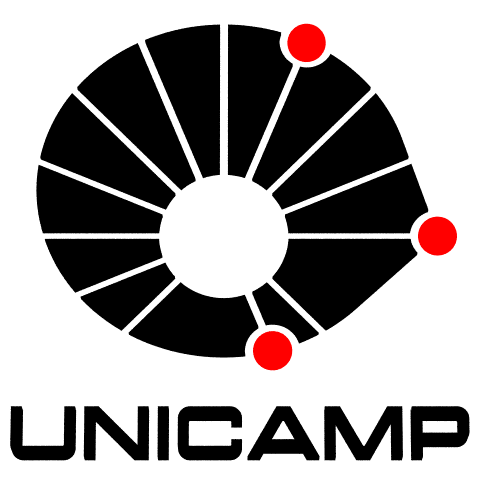
\includegraphics[scale=0.18]{image/LogoUnicamp}
\end{figure} 
%
\vspace*{10pt}
%\text{ }\\[7 cm]
\textbf{\LARGE Exercício de Fixação de Conceitos 2} \\ \vspace{12pt}
\textbf{\large EA072 - Inteligência Artificial em Aplicações Industriais}
\vspace*{72pt}

Gustavo \textbf{CIOTTO PINTON} - \textbf{RA 117136}
 

Campinas, \today

\end{center}
\end{titlepage}

\newpage
%  
% {\large 
%     \centerline{\textbf{Exercício de Fixação de Conceitos 1}}
%     \centerline{Gustavo Ciotto Pinton - 117136}
%     \centerline{EA072 - Inteligência Artificial em Aplicações Industriais}
% }

			\section {Seleção de variáveis empregando filtros e \textit{wrappers}}
			
			\begin{enumerate}
			  \item A quantidade de dados e de variáveis de entrada podem representar
			  verdadeiros obstáculos no treinamento e validação dos pesos sinápticos de
			  redes neurais, principalmente ao que se refere aos recursos disponíveis de
			  processamento. Sendo assim, algoritmos e técnicas que possam ser capazes de
			  determinar o grau de importância das variáveis em relação à saída e
			  distinguir os dados mais pertinentes tornam-se indispensáveis a essas
			  operações. Destacam-se duas técnicas: a primeira, a chamada técnica
			  \textit{\textbf{filter}}, busca a classificar as variáveis de acordo com
			  algum critério, seja ele a \textit{correlação} ou a \textit{informação mútua}
			  entre as variáveis de entrada \(\boldsymbol{x_j} \) e as saídas
			  \(\boldsymbol{y_i} \). Tais técnicas independem do modelo de predição e são
			  aplicadas durante a fase de pré-processamento.  A segunda, chamada
			  \textit{\textbf{wrapper}}, utiliza uma máquina de aprendizado qualquer como
			  uma caixa preta e avalia os subconjuntos de variáveis de acordo com suas
			  respectivas qualidades de predição. Tais características podem impor algumas
			  dificuldades a essa últmia técnica, à medida que a avaliação dos resultados
			  de predição pode não ser tão trivial e o método de construção dos
			  subconjuntos pode apresentar uma complexidade elevada. Destacam-se, portanto,
			  os métodos de \textit{forward selection} e \textit{backward elimination}.
			  
			  
			  \item Seja \(\mathbb{S}\) o conjunto de variáveis de entrada cujo efeito na
			  saída do modelo \(\boldsymbol{\hat{y}_k}\) seja pertinente em relação à saída esperada
			  \(\boldsymbol{y_k}\).  A abordagem de \textit{forward selection} consiste a
			  aumentar progressivamente \(\mathbb{S}\), à medida que uma variável se mostre
			  importante ao modelo. A importância de uma variável pode ser determinada
			  através de alguns critérios, como por exemplo o cálculo de 
			  \(J\left(\mathbb{S} \cup \{ x_i \} \right) = \sum_{k=1}^{m}(\boldsymbol{\hat{y}_k} -
			  \boldsymbol{y_k})^2 \), sendo \(x_i\) um variável canditata à
			  inserção. Neste caso, compara-se \(J\left(\mathbb{S} \cup \{ x_i \} \right)\) e
			  \(J\left(\mathbb{S} \right)\) e, caso o efeito dessa variável seja positivo, isto é,
			  \(J\left(\mathbb{S} \cup \{ x_i \} \right)\) menor, a acrescentamos em \(\mathbb{S}\). Para
			  \textit{forward selection}, \(\mathbb{S}\) começa vazio.
			  
			  A abordagem de  \textit{backward elimination}, por sua vez, elimina de \(\mathbb{S}\)
			  gradativamente as variáveis menos pertinentes ao modelo. \(\mathbb{S}\) é, portanto,
			  inicializado com todas as variáveis. Analogamente ao caso anterior, pode-se
			  calcular \(J\left(\mathbb{S} \setminus \{ x_i \} \right)\) e compará-lo com
			  \(J\left(\mathbb{S}\right)\). Caso \(J\left(\mathbb{S} \setminus \{ x_i \} \right)\) seja
			  inferior, elimina-se de \(\mathbb{S}\) a variável \(\{x_i\}\).
			  
			  As duas abordagens acima não garantem a melhor combinação de entradas pelo
			  fato da possível existência de \textit{mínimos locais} da função
			  \(J(\mathbb{T})\), a função que associa o erro com as variáveis presentes no
			  conjunto \(\mathbb{T}\). Dependendo das condições e ordem de verificação das
			  variáveis \(x_i\), o método pode tender a diferentes mínimos, que podem ser
			  eventualmente os melhores ou não.
			
			
			  \item \begin{enumerate}
			    \item A tabela \ref{tab:estat_tab} a seguir descreve algumas características estatísticas da série temporal. Todos os valores foram calculador através do MATLAB. Além delas, a série é formada por \(3180\) entradas, sendo compostas pelos dados de todos os meses de 1749 até 2013. 
			    
			    \begin{table}[h]
				    \centering
					\caption{\label{tab:estat_tab} Características da série temporal}
					\begin{tabular}{|c | c |}
						\hline
						Propriedades & Valor \\	\hhline{|=|=|}
						Média & \(51.9949\) \\ \hline 
						Valor máximo & \(253.8\) \\ \hline 
						Valor mínimo & \(0\) \\ \hline 			
						Desvio padrão & \(41.116\) \\ \hline 			
					\end{tabular}	    
			    \end{table}    
			    
			    \item Para o \textit{filtro linear}, as execuções de 
			    \textit{filtro\_lin(dados1.mat)} e \textit{filtro\_nlin(dados1.mat)}
			    resultam nas figuras \ref{fig:filtro_lin} e \ref{fig:filtro_nlin},
			    respectivamente.
			    
				\begin{figure}
				
				\centering
				
					\begin{subfigure}{.5\textwidth}
					  \centering
					  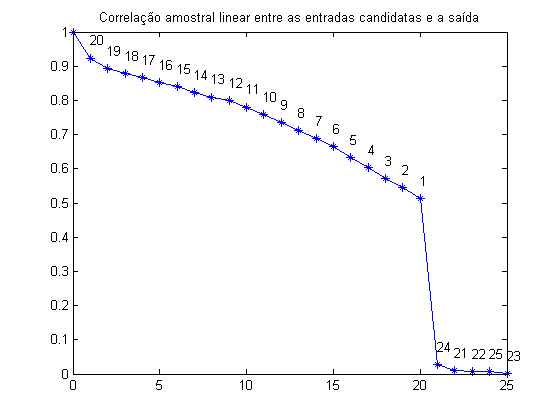
\includegraphics[width=1\linewidth]{image/filtro_lin}
					  \caption{Resultado do \textit{filtro linear}.}
					  \label{fig:filtro_lin}
					\end{subfigure}%
					\begin{subfigure}{.5\textwidth}
					  \centering
					  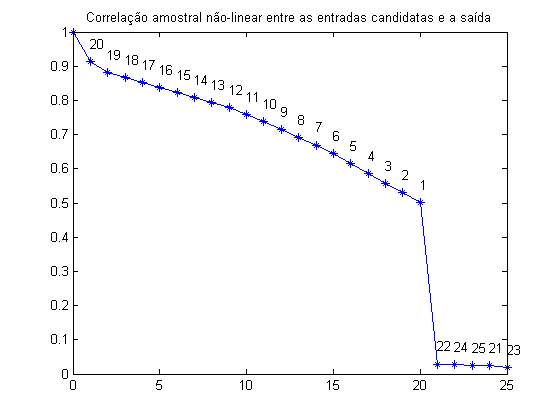
\includegraphics[width=1\linewidth]{image/filtro_nlin}
					  \caption{Resultado do \textit{filtro não linear}.}
					  \label{fig:filtro_nlin}
				\end{subfigure}
				
				\caption{Resultados das execuções das funções de filtro.}
				\end{figure}
				
				
			\FloatBarrier
				
			Conclui-se portanto que as variáveis de \(1\) a \(20\) apresentam as maiores
			correlações, tanto a linear \(R_{linear}\) quanto a não linear \(R_{nlinear}\),
			em relação à saída, sendo a \(20^a\) a mais correlata. A ordem de relevância em
			que elas aparecem também é a mesma, isto é, a sêquencia decrescente de 20 até 1
			é observada em ambos os casos, e a maior diferença percentual entre
			\(R_{linear}\) e \(R_{nlinear}\) é de \(3.12\%\), correspondente à \(13^a\)
			variável.
				
				\vspace{12pt}
				
			Observa-se ainda que as variáveis 21 até 25 apresentam \(R_{linear}\) e
			\(R_{nlinear}\) são muito inferiores em relação aos valores das outras varíaveis
			e que a sua ordem de relevância é diferente: para o filtro \textit{linear} temos
			a sequência 24, 21, 22, 25 e 23, enquanto que para o \textit{não linear} obtemos
			22, 24, 25, 21 e 23.
			
			
			\item 
			\label{item:forwsunspot}
			Para o método \textbf{\textit{forward selection}}\footnote{As
			imagens referentes a estas execuções encontram-se na figura \ref{fig:forw}
			na seção \textbf{Anexos} no fim do documento}, obtem-se para as 5 execuções os seguintes dados:
			
			\begin{table}[H]
				    \centering
				    \footnotesize
					\caption{\label{tab:forward1_sunspot} Resultados da execução
					\textit{\textbf{1}}.}
				    \vspace{-6pt}
					\begin{tabular}{|c | c | c | c | c | c | c | c | c | c | c | c | c | c|}
					\hline
					Entradas & 20 & 18 & 17 & 3 & 12 & 19 & 15 & 1 & 16 & 11 & 23 & 5 & 7 \\
					\hline
					Erro mínimo & \multicolumn{13}{c|}{\(1.1765\)}  \\ \hline
					No. de Variáveis & \multicolumn{13}{c|}{\(13\)}  \\
					\hline
					
					\end{tabular}	    
			    \end{table}    

		\vspace{-12pt}

			\begin{table}[H]
				    \centering
					\caption{\label{tab:forward2_sunspot} Resultados da execução
					\textit{\textbf{2}}.}
					\footnotesize
				    \vspace{-6pt}
					\begin{tabular}{|c | c | c | c | c | c | c | c | c | c | c | c | c | c | c |
					c|}
					\hline
					Entradas & 20 & 18 & 17 & 3 & 12 & 19 & 15 & 1 & 10 & 5 & 22 & 7 & 21 & 25 & 16 \\
					\hline
					Erro mínimo & \multicolumn{15}{c|}{\(1.1745\)}  \\ \hline
					No. de Variáveis & \multicolumn{15}{c|}{\(15\)}  \\
					\hline
					
					\end{tabular}	    
			    \end{table}     

		\vspace{-12pt}

			\begin{table}[H]
				    \centering
				    \footnotesize
					\caption{\label{tab:forward3_sunspot} Resultados da execução
					\textit{\textbf{3}}.}
				    \vspace{-6pt}
					\begin{tabular}{|c | c | c | c | c | c | c | c | c | c | c | c | c | c | c|}
					\hline
					Entradas & 20 & 18 & 17 & 3 & 12 & 15 & 19 & 1 & 16 & 23 & 5 & 10 & 13 & 24 \\
					\hline
					Erro mínimo & \multicolumn{14}{c|}{\(1.1727\)}  \\ \hline
					No. de Variáveis & \multicolumn{14}{c|}{\(14\)}  \\
					\hline
					
					\end{tabular}	    
			    \end{table}     

		\vspace{-12pt}

			\begin{table}[H]
				    \centering
				    \footnotesize
					\caption{\label{tab:forward4_sunspot} Resultados da execução
					\textit{\textbf{4}}.}
				    \vspace{-6pt}
					\begin{tabular}{|c | c | c | c | c | c | c | c | c | c | c | c | c | c | c
					| c|}
					\hline
					Entradas & 20 & 18 & 17 & 3 & 12 & 15 & 19 & 1 & 16 & 10 & 5 & 23 & 24 & 13 & 21 \\
					\hline
					Erro mínimo & \multicolumn{15}{c|}{\(1.1707\)}  \\ \hline
					No. de Variáveis & \multicolumn{15}{c|}{\(15\)}  \\
					\hline
					
					\end{tabular}	    
			    \end{table} 
			    
		\vspace{-12pt}

			\begin{table}[H]
				    \centering
				    \footnotesize
					\caption{\label{tab:forward5_sunspot} Resultados da execução
					\textit{\textbf{5}}.}
				    \vspace{-6pt}
					\begin{tabular}{|c | c | c | c | c | c | c | c | c | c | c | c | c|}
					\hline
					Entradas & 20 & 18 & 17 & 3 & 12 & 19 & 15 & 1 & 10 & 11 & 5 & 7 \\
					\hline
					Erro mínimo & \multicolumn{12}{c|}{\(1.1768\)}  \\ \hline
					No. de Variáveis & \multicolumn{12}{c|}{\(12\)}  \\
					\hline
					
					\end{tabular}	    
			    \end{table} 
	
			    \FloatBarrier
	
		Considerando somente as primeiras cinco variáveis selecionadas em cada execução,
		percebe-se que, em realidade, elas são todas iguais: 20, 18, 17, 3 e 12, nessa
		sequência. Na sexta posição, encontra-se a variável 19 (3 ocasiões) ou a 15 (2
		ocasiões) e na sétima, a variável 1. À partir dessa posição, as entradas
		selecionadas variam a cada iteração.
		
		\vspace{12pt}	
	
		Para o método \textbf{\textit{backward elimination}}\footnote{As
			imagens referentes a estas execuções encontram-se na figura \ref{fig:back}
			na seção \textbf{Anexos} no fim do documento}, obtem-se:
			
			\begin{table}[H]
				    \centering
				    \footnotesize
					\caption{\label{tab:backward1_sunspot} Resultados da execução
					\textit{\textbf{1}}.}
				    \vspace{-6pt}
					\begin{tabular}{|c | c | c | c | c | c | c | c | c | c | c | c | c | c | c |
					c|}
					\hline
					Entradas & 23 & 25 & 24 & 5 & 22 & 16 & 21 & 1 & 18 & 15 & 19 & 12 & 3 & 17 & 20  \\
					\hline
					Erro mínimo & \multicolumn{15}{c|}{\(1.1711\)}  \\ \hline
					No. variáveis restantes & \multicolumn{15}{c|}{\(15\)}  \\
					\hline
					
					\end{tabular}	    
			    \end{table}    

		\vspace{-12pt}

			\begin{table}[H]
				    \centering
				    \footnotesize
					\caption{\label{tab:backward2_sunspot} Resultados da execução
					\textit{\textbf{2}}.}
				    \vspace{-6pt}
					\begin{tabular}{|c | c | c | c | c | c | c | c | c | c | c | c | c | c | c
					|}
					\hline
					Entradas & 8 & 25 & 11 & 7 & 5 & 16 & 1 & 15 & 18 & 19 & 12 & 3 & 17 & 20  \\
					\hline
					Erro mínimo & \multicolumn{14}{c|}{\(1.1717\)}  \\ \hline
					No. variáveis restantes & \multicolumn{14}{c|}{\(14\)}  \\
					\hline
					
					\end{tabular}	    
			    \end{table}       

		\vspace{-12pt}

			\begin{table}[H]
				    \centering
				    \footnotesize
					\caption{\label{tab:backward3_sunspot} Resultados da execução
					\textit{\textbf{3}}.}
				    \vspace{-6pt}
					\begin{tabular}{|c | c | c | c | c | c | c | c | c | c | c | c | c | c | c |
					c |}
					\hline
					Entradas & 8 & 7 & 23 & 21 & 5 & 16 & 11 & 1 & 18 & 15 & 19 & 12 & 3 & 17 & 20  \\
					\hline
					Erro mínimo & \multicolumn{15}{c|}{\(1.1744\)}  \\ \hline
					No. variáveis restantes & \multicolumn{15}{c|}{\(15\)}  \\
					\hline
					
					\end{tabular}	    
			    \end{table}       
		\vspace{-12pt}

			\begin{table}[H]
				    \centering
				    \footnotesize
					\caption{\label{tab:backward4_sunspot} Resultados da execução
					\textit{\textbf{4}}.}
				    \vspace{-6pt}
					\begin{tabular}{|c | c | c | c | c | c | c | c | c | c  | c | c | c | c | c
					| c | c | }
					\hline
					Entradas & 6 & 21 & 7 & 8 & 10 & 24 & 16 & 25 & 1 & 18 & 15 & 19 & 12 & 3 & 17 & 20  \\
					\hline
					Erro mínimo & \multicolumn{16}{c|}{\(1.1733\)}  \\ \hline
					No. variáveis restantes & \multicolumn{16}{c|}{\(16\)}  \\
					\hline
					
					\end{tabular}	    
			    \end{table}  	
			    
		\vspace{-12pt}

			\begin{table}[H]
				    \centering
				    \footnotesize
					\caption{\label{tab:backward5_sunspot} Resultados da execução
					\textit{\textbf{5}}.}
				    \vspace{-6pt}
					\begin{tabular}{|c | c | c | c | c | c | c | c | c | c | c | c | c | c | c|}
					\hline
					Entradas & 7 & 21 & 13 & 16 & 5 & 10 & 1 & 18 & 15 & 19 & 3 & 12 & 17 & 20   \\
					\hline
					Erro mínimo & \multicolumn{14}{c|}{\(1.1748\)}  \\ \hline
					No. variáveis restantes & \multicolumn{14}{c|}{\(14\)}  \\
					\hline
					
					\end{tabular}	    
			    \end{table}  	
	
			    \FloatBarrier	
	
		Observa-se que o número de variáveis restantes para as execuções do
		\textit{backward elimination} é ligeiramente superior em relação ao método
		anterior, apresentando uma média de 15 variáveis escolhidas contra
		aproximadamente 14 do \textit{forward selection}. A média do erro quadrado
		médio na construção do modelo é inferior para \textit{backward
		elimination}: 1.1731 contra 1.1742. Nota-se ainda que algumas variáveis foram
		escolhidas em todas as execuções de ambos, sendo elas, por exemplo, a 20, 17,
		3, 12 e a 15.
	
		 \item Entradas que possuem as maiores correlações não são as primeiras a
		 serem adicionadas ao modelo pela presença de \textit{redundância} entre elas.
		 Se uma variável é altamente correlata com uma outra, eu não precisaria, em
		 príncipio, conhecer as duas, já que a partir de um única, eu sou capaz de
		 determinar a outra. Em outras palavras, variáveis \textit{redundantes}
		 adicionam pouca informação ao sistema. Por exemplo, a correlação entre as
		 variáveis 20 e 19 do arquivo \texttt{dados1.mat} vale 0.9239 (valor obtido
		 pelo comando \texttt{corr(X(:,20), X(:,19))} do MATLAB). Isso signfica que se
		 \(X_{20}\) é alto, então \(X_{19}\) também o é e, portanto, nenhuma outra
		 informação é adicionada ao modelo. É por essa razão que nas execuções acima,	
		 \(X_{20}\) é escolhida inicialmente e \(X_{19}\), só depois de algumas
		 iterações.
		 
		\item Variáveis de baixa correlação com a saída podem proporcionar um grande poder
		de separação, se consideradas juntamente com outras\footnote{No artigo \textit {[ Guyon,  I.;  Elisseeff,  A.
		“An  introduction  to  variable  and feature selection”, Journal of Machine
		Learning Resear ch, vol. 3, pp. 1157 - 1182 2003 ]}, o autor dá um exemplo dessa
		afirmação na seção 3.3.}. Desta maneira, as variáveis de menor correlação são
		separadas mais facilmente em relação àquelas de maior correlação, permitindo
		assim a detecção de classes com maior precisão. Em outras palavras, entradas
		mais próximas das variáveis de baixa correlação podem ser classificadas mais
		facilmente.

		 \item As variáveis geradas aleatoriamente (\( X_{21} \cdots X_{25} \))
		 apresentam correlações em relação à saída praticamente nulas (os resultados
		 de \texttt{corr (X(:,21), S)} \ldots  ~\texttt{corr (X(:,25), S)} estão
		 mostrados na tabela \ref{tab:corr.aleat.}). Dessa maneira, elas são
		 escolhidas em ambos os modelos pelos mesmos motivos daqueles discutidos nos
		 dois itens anteriores (\textit{redundância} e \textit{poder de separação}).
		 
		 \begin{table}[H]
				    \centering
					\caption{\label{tab:corr.aleat.} Correlação das variáveis
					aleatórias execução 1 do \textit{forward selection}.}
					\begin{tabular}{| c | c |}
					
					\hline
					Variável \(X_i \) & \texttt{corr (X(:,i), S)} \\ \hline \hline
					\(X_{21}\) & 0.001347309212350 \\ \hline
					\(X_{22}\) & 0.011839959350690 \\ \hline
					\(X_{23}\) & -0.037287334573179 \\ \hline
					\(X_{24}\) & -0.007005116183944 \\ \hline
					\(X_{25}\) & 0.001963170472808 \\ \hline
					
					
					\end{tabular}	    
			    \end{table}  	
	
			    \FloatBarrier
		 
		\end{enumerate}
		
		\item \begin{enumerate}
		  \item O arquivo \texttt{wineq.mat} é composto por duas estruturas de dados.
		  A primeira, matriz \(X_{1593 \times 11}\), possui 11 colunas, correpondentes
		  a cada uma das variáveis de entrada, e 1593 linhas, simbolizando 1593 dados
		  disponíveis. De acordo com o \textit{website} de onde tais dados foram
		  retirados, essas variáveis correspondem a diversas propriedades que podem
		  ser extraídas de um vinho, sendo elas \textit{fixed acidity},
		  \textit{volatile acidity}, \textit{citric acid}, \textit{residual sugar},
		  \textit{chlorides}, \textit{free sulfur dioxide}, \textit{total sulfur
		  dioxide}, \textit{density}, \textit{pH}, \textit{sulphates} e
		  \textit{alcohol}. A tabela abaixo mostra algumas características dessas
		  propriedades.
		  
		  \begin{table}[H]
			    \centering
				\caption{\label{tab:wineq.mat} Informações correpondentes às variáveis de
				\texttt{wineq.mat}.}
				\begin{tabular}{| c | c |  c | c | c |}
				
				\hline
				Variável & Média & Max. & Min. & \textit{Standard Deviation} \\ \hhline{|=|=|=|=|=|} 
				\textit{fixed acidity} & 0.52324 & 1 & 0.28931 &
				0.10932 \\ \hline \textit{volatile acidity} & 0.33385 & 1 & 0.075949 & 0.11333 \\ \hline
				 \textit{citric acid} & 0.27116 & 1 & 0 & 0.19495 \\ \hline
				 \textit{residual sugar} & 0.16374 & 1 & 0.058065 & 0.090957 \\ \hline
				 \textit{chlorides} & 0.14321 & 1 & 0.01964 & 0.077153 \\ \hline
				 \textit{free sulfur dioxide} & 0.2205 & 1 & 0.013889 & 0.14537 \\ \hline
				 \textit{total sulfur dioxide}& 0.16052 & 1 & 0.020761 & 0.11379 \\ \hline
				 \textit{density} & 0.022051 & 1 & 0.0098643 & 0.096464 \\ \hline
				  \textit{pH} & 0.82574 & 1 & 0.68329 & 0.038451 \\ \hline
				 \textit{sulphates}& 0.32903 & 1 & 0.165 & 0.084846 \\ \hline
				 \textit{alcohol} & 0.69949 & 1 & 0.56376 & 0.071404 \\ \hline
				
				\end{tabular}	    
		    \end{table} 
		    
		    Para a saída encontra-se:
		    
		    \begin{table}[H]
			    \centering
				\caption{\label{tab:wineqSaida.mat} Informações correpondentes à saída
				de
				\texttt{wineq.mat}.}
				\begin{tabular}{| c | c |  c | c | c |}
				
				\hline
				Variável & Média & Max. & Min. & \textit{Standard Deviation} \\ \hhline{|=|=|=|=|=|} 
				Saída & 0.70425 & 1 & 0.375 & 0.10101 \\ \hline
				
				\end{tabular}	    
		    \end{table} 
		    
		    \item As execuções de \texttt{filtro\_lin('dados2.mat')} e
		    \texttt{filtro\_nlin('dados2.mat')} são mostradas na figuras
		    \ref{fig:filtro_lin2} e \ref{fig:filtro_nlin2} a seguir.
		    
		    \begin{figure}[H]
				
				\centering
				
					\begin{subfigure}{.5\textwidth}
					  \centering
					  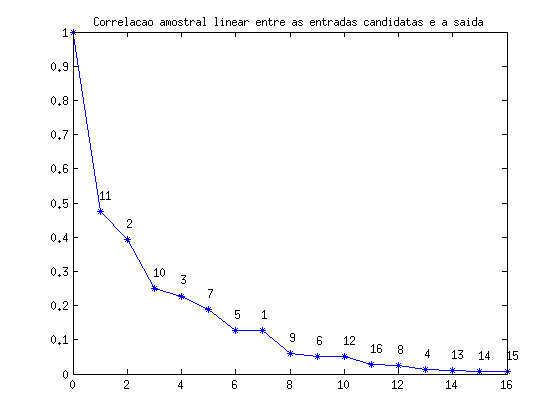
\includegraphics[width=1\linewidth]{image/filtro_lin2}
					  \caption{Resultado do \textit{filtro linear}.}
					  \label{fig:filtro_lin2}
					\end{subfigure}%
					\begin{subfigure}{.5\textwidth}
					  \centering
					  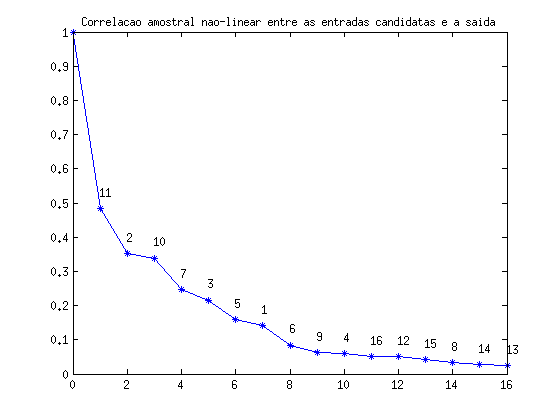
\includegraphics[width=1\linewidth]{image/filtro_nlin2}
					  \caption{Resultado do \textit{filtro não linear}.}
					  \label{fig:filtro_nlin2}
				\end{subfigure}
				
				\caption{Resultados das execuções das funções de filtro.}
				\end{figure}
				
			\FloatBarrier
			
			Neste caso, observa-se uma maior diferença entre as filtragens linear e não
			linear em relação ao estudo de caso anterior. Percebe-se inicialmente que a
			correlação da variável mais correlata (\(<0.5\)) aqui é muito inferior
			àquela mais correlata (\(>0.9\)) para os dados referentes aos
			\textit{Sunspots}. 
			
			\vspace{12pt}
			
			A ordem decrescente de correlação em que as variáveis aparecem também muda do
			caso linear para o não linear. A tabela seguinte evidencia
			esta afirmação. \(\Delta =  \frac {\left( R_{nlin} - R_{lin}
			\right)}{R_{nlin}} \), onde \(R\) é o valor da correlação linear ou não
			linear, representa a variação percentual entre as respectivas correlações.
			
			\begin{table}[H]
			    \centering
			    \footnotesize
				\caption{\label{tab:ordem} Ordens de aparição das variáveis.}
				\begin{tabular}{| c | c |  c | c | c | c | c |  c | c | c | c | c |  c | c |
				c | c | c |}
				\hline
				 & \multicolumn{16}{|c|}{Ordem} \\
				\hhline{|=|=|=|=|=|=|=|=|=|=|=|=|=|=|=|=|=|} 
				\(V_{lin}\) & 11 & 2 & 10 & 3 & 7 & 5 & 1 & 9 & 6 & 12 &
				16 & 8 & 4 & 13 & 14 & 15 \\ \hline 
				
				\(V_{nlin}\) &  11 & 2 & 10 & 7 & 3 & 5 & 1 & 6 & 9 & 4 
				& 16 & 12 & 15 & 8 & 14 & 13 \\ \hline 
				
				\(\Delta\) & 0.01 & -0.12 & 0.26 & 0.07 & 0.13 & 0.2 &
				0.11 & 0.31 & 0.18 & 0.16 & 0.46 & 0back.5 & 0.68 & 0.73 & 0.75 & 0.72 \\
				\hline
				\end{tabular}	    
		    \end{table} 

			
			\FloatBarrier
			
			Observa-se que a ordem muda sobretudo no fim da sequência, onde as
			variações percentuais são superiores.
			
			\item 
			\label{item:forwwineq}
			Para o método \textbf{\textit{forward selection}}\footnote{As
			imagens referentes a estas execuções encontram-se na figura \ref{fig:forw2}
			na seção \textbf{Anexos} no fim do documento}, obtem-se para as 5
			execuções os seguintes dados:
			
			\begin{table}[H]
					\setlength\tabcolsep{4pt}
					\begin{minipage}{0.48\textwidth}
					    \centering
					    \footnotesize
						\caption{\label{tab:forward1_wine} Resultados da execução
						\textit{\textbf{1}}.}
					    \vspace{-6pt}
						\begin{tabular}{|c | c | c | c | c | c | c | c | c |}
						\hline
						Entradas & 11 & 2 & 10 & 7 & 5 & 9 & 6 & 16 \\
						\hline
						Erro mínimo & \multicolumn{8}{c|}{\(1.0484\)}  \\ \hline
						No. de Variáveis & \multicolumn{8}{c|}{\(8\)}  \\
						\hline
						
						\end{tabular}
					\end{minipage}	    
					\begin{minipage}{0.48\textwidth}
					    \centering
						\caption{\label{tab:forward2_wine} Resultados da execução
						\textit{\textbf{2}}.}
						\footnotesize
					    \vspace{-6pt}
						\begin{tabular}{|c | c | c | c | c | c | c | c | c | c |}
						\hline
						Entradas & 11 & 2 & 10 & 7 & 5 & 9 & 6 & 13 & 14 \\
						\hline
						Erro mínimo & \multicolumn{9}{c|}{\(1.0491\)}  \\ \hline
						No. de Variáveis & \multicolumn{9}{c|}{\(9\)}  \\
						\hline
						
						\end{tabular}	
					\end{minipage}	    
			    \end{table}     

		\vspace{-12pt}

			\begin{table}[H]
					\setlength\tabcolsep{4pt}
					\begin{minipage}{0.48\textwidth}
					    \centering
					    \footnotesize
						\caption{\label{tab:forward3_wine} Resultados da execução
						\textit{\textbf{3}}.}
					    \vspace{-6pt}
						\begin{tabular}{|c | c | c | c | c | c | c | c | c |}
						\hline
						Entradas & 11 & 2 & 10 & 7 & 5 & 9 & 6 & 13 \\
						\hline
						Erro mínimo & \multicolumn{8}{c|}{\(1.0495\)}  \\ \hline
						No. de Variáveis & \multicolumn{8}{c|}{\(8\)}  \\
						\hline
						
						\end{tabular}	    
					\end{minipage}	    
					\begin{minipage}{0.48\textwidth}
					    \centering
					    \footnotesize
						\caption{\label{tab:forward4_wine} Resultados da execução
						\textit{\textbf{4}}.}
					    \vspace{-6pt}
						\begin{tabular}{|c | c | c | c | c | c | c | c | c|}
						\hline
						Entradas & 11 & 2 & 10 & 7 & 5 & 9 & 6 & 14 \\
						\hline
						Erro mínimo & \multicolumn{8}{c|}{\(1.0509\)}  \\ \hline
						No. de Variáveis & \multicolumn{8}{c|}{\(8\)}  \\
						\hline
						
						\end{tabular}
					\end{minipage}	    
			    \end{table} 
			    
			\vspace{-12pt}

			\begin{table}[H]
				    \centering
				    \footnotesize
					\caption{\label{tab:forward5_wine} Resultados da execução
					\textit{\textbf{5}}.}
				    \vspace{-6pt}
					\begin{tabular}{|c | c | c | c | c | c | c | c | c|}
					\hline
					Entradas & 11 & 2 & 10 & 7 & 5 & 9 & 6 & 13 \\
					\hline
					Erro mínimo & \multicolumn{8}{c|}{\(1.0509\)}  \\ \hline
					No. de Variáveis & \multicolumn{8}{c|}{\(8\)}  \\
					\hline
					
					\end{tabular}	    
			    \end{table} 
	
			    \FloatBarrier
			    
			Para o método \textbf{\textit{backward elimination}}\footnote{As
			imagens referentes a estas execuções encontram-se na figura \ref{fig:back2}
			na seção \textbf{Anexos} no fim do documento}, obtem-se:
			
			\begin{table}[H]
					\setlength\tabcolsep{4pt}
					\begin{minipage}{0.48\textwidth}
					    \centering
					    \footnotesize
						\caption{\label{tab:backward1_wine} Resultados da execução
						\textit{\textbf{1}}.}
					    \vspace{-6pt}
						\begin{tabular}{|c | c | c | c | c | c | c | c | c |}
						\hline
						Entradas & 13 & 6 & 9 & 5 & 7 & 10 & 2 & 11 \\
						\hline
						Erro mínimo & \multicolumn{8}{c|}{\(1.0496\)}  \\ \hline
						No. de Variáveis & \multicolumn{8}{c|}{\(8\)}  \\
						\hline
						
						\end{tabular}
					\end{minipage}	    
					\begin{minipage}{0.48\textwidth}
					    \centering
						\caption{\label{tab:backward2_wine} Resultados da execução
						\textit{\textbf{2}}.}
						\footnotesize
					    \vspace{-6pt}
						\begin{tabular}{|c | c | c | c | c | c | c | c | c | c |}
						\hline
						Entradas & 15 & 3 & 14 & 9 & 5 & 7 & 10 & 2 & 11  \\
						\hline
						Erro mínimo & \multicolumn{9}{c|}{\(1.0558\)}  \\ \hline
						No. de Variáveis & \multicolumn{9}{c|}{\(9\)}  \\
						\hline
						
						\end{tabular}	
					\end{minipage}	    
			    \end{table}     

		\vspace{-12pt}

			\begin{table}[H]
					\setlength\tabcolsep{4pt}
					\begin{minipage}{0.48\textwidth}
					    \centering
					    \footnotesize
						\caption{\label{tab:backward3_wine} Resultados da execução
						\textit{\textbf{3}}.}
					    \vspace{-6pt}
						\begin{tabular}{|c | c | c | c | c | c | c | c | c | c | c |}
						\hline
						Entradas & 15 & 12 & 3 & 6 & 9 & 5 & 7 & 10 & 2 & 11  \\
						\hline
						Erro mínimo & \multicolumn{10}{c|}{\(1.0532\)}  \\ \hline
						No. de Variáveis & \multicolumn{10}{c|}{\(10\)}  \\
						\hline
						
						\end{tabular}	    
					\end{minipage}	    
					\begin{minipage}{0.48\textwidth}
					    \centering
					    \footnotesize
						\caption{\label{tab:backward4_wine} Resultados da execução
						\textit{\textbf{4}}.}
					    \vspace{-6pt}
						\begin{tabular}{|c | c | c | c | c | c | c | c | c| c| c|}
						\hline
						Entradas & 3 & 1 & 14 & 6 & 9 & 5 & 7 & 10 & 2 & 11 \\
						\hline
						Erro mínimo & \multicolumn{10}{c|}{\(1.0548\)}  \\ \hline
						No. de Variáveis & \multicolumn{10}{c|}{\(10\)}  \\
						\hline
						
						\end{tabular}
					\end{minipage}	    
			    \end{table} 
			    
			\vspace{-12pt}

			\begin{table}[H]
				    \centering
				    \footnotesize
					\caption{\label{tab:backward5_wine} Resultados da execução
					\textit{\textbf{5}}.}
				    \vspace{-6pt}
					\begin{tabular}{|c | c | c | c | c | c | c | c | c| c|}
					\hline
					Entradas & 12 & 6 & 14 & 9 & 5 & 7 & 10 & 2 & 11 \\
					\hline
					Erro mínimo & \multicolumn{9}{c|}{\(1.0497\)}  \\ \hline
					No. de Variáveis & \multicolumn{9}{c|}{\(9\)}  \\
					\hline
					
					\end{tabular}	    
			    \end{table} 
	
			    \FloatBarrier
		     
		     Observa-se que para a técnica de \textit{forward selection} as primeiras
		     sete entradas selecionadas foram as mesmas para as 5 execuções, sendo
		     elas a 11, 2, 10, 7, 5, 9 e 6. As restantes escolhidas fazem parte das
		     entradas aleatórias, calculadas para cada execução. Em média, foram
		     escolhidas 8 variáveis e produziu-se um erro de 1.04976.
		     
		     \vspace{12pt}
		     
		     Em relação à técnica de \textit{backward elimination}, as mesmas
		     variáveis citadas no parágrafo anterior estiveram presentes, com exceção
		     à 6, em que esteve ausente somente na execução 2. Foram selecionadas, em
		     média, um número maior de variáveis, 9, e um erro superior, 1.05262. As
		     variáveis restantes foram escolhidas dentre as geradas aleatoriamente.
		     
		     \vspace{12pt}
		     
		     Finalmente, as váriaveis que foram escolhidas nos primeiros lugares na
		     \textit{forward selection} seriam eliminadas por último na
		     \textit{backward elimination}, confirmando assim um certo nível de
		     semelhância nos resultados das duas técnicas.
		     
		\end{enumerate}
\end{enumerate}
		  


\section{Séries temporais e a tarefa de predição}


\setcounter{subsection}{-1}
\subsection{Normalização dos dados}

	De acordo com enunciado disponibilizado, os dados devem ser normalizados de
	maneira a obter média nula e desvio padrão unitário. Entradas que excursionam
	em intervalos muito extensos prejudicam o desempenho das redes neurais MLP.
	
	\vspace{12pt}
	
	Sendo assim, faremos uso da seguinte equação para atingir as características
	necessárias:
	
	\begin{equation}
	X_i = \frac{V_i - \hat{\mu}}{\hat{\sigma}}
	\end{equation}
	
	em que \(\hat{\mu}\) é a média de todas as entradas (calcula através de
	\texttt{mean(dengue\_SP)}) e \(\hat{\sigma}\) é o estimador do desvio padrão
	(calculado por \texttt{std(dengue\_SP)}). Obtem-se, assim, um novo vetor cuja
	média e variância valem, respectivamente, \(1.8288\times10^{-16}\) e 1. A
	figura à seguir mostra um histograma dos dados normalizados. Observa-se que a
	maioria dos dados encontram-se na vizinhança de 0, mas há uma quantidade
	razoável deles superior à unidade, correspondentes aos períodos de chuva, onde
	há, naturalmente, mais casos da doença.
	
	\begin{figure}[H]
			\centering
			  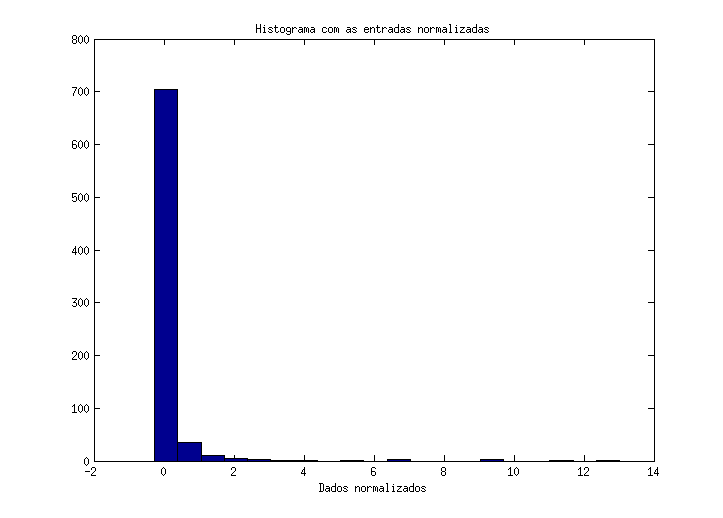
\includegraphics[width=0.65\textwidth]{image/hist_normalizados}
			  \caption{Dados normalizados.} 
			  \label{hist3}
	\end{figure}
	
	\FloatBarrier

\subsection{Variáveis participantes do modelo - Filtro de correlação}
 \label{sec:corr}

A fim de obter um resultado mais representativo nos preditores a serem
realizados, aplica-se um filtro de correlações nas 20 variáveis que inicialmente
foram propostas para determinar a precvisão do número de casos de dengue para a
próxima semana. Para isso, usamos o programa \texttt{calc\_corr2.m},
disponibilizado pelo professor. Obtem-se o gráfico mostrado na figura
\ref{fig:corr_variavel} a seguir:

	\begin{figure}[H]
			\centering
			  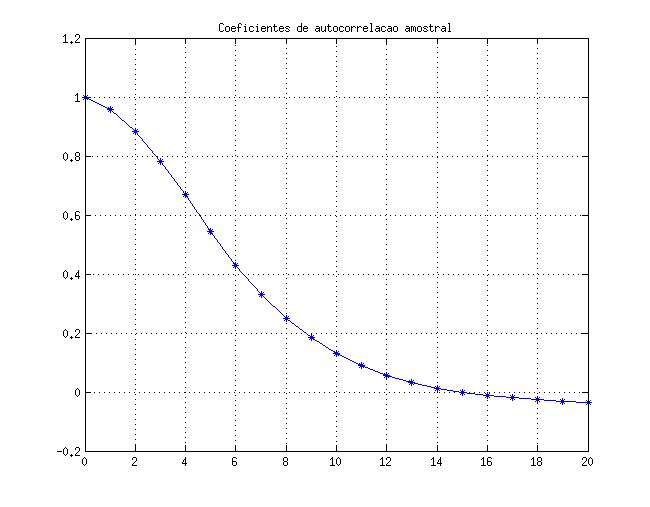
\includegraphics[width=0.60\textwidth]{image/corr_variaveis_preditor}
			  \caption{Correlação das 20 variavés escolhidas como entrada.} 
			  \label{fig:corr_variavel}
	\end{figure}
	
	\FloatBarrier
	
Observa-se neste gráfico que as cinco primeiras variáveis utilizadas no modelo
são as mais correlatas à saída. Em termos numéricos, as variáveis a partir da
sexta apresentam correlações inferiores a 0.5. Conclui-se, portanto, que em
termos de pertinência, as cinco variáveis iniciais são as mais importantes para
compor o valor a ser predito.

\subsection{Síntese de um preditor linear}
 
Para esta etapa, define-se \(M = 5\) a dimensão do espaço de entrada (consultar
seção \ref{sec:corr}) e \(R = 1\), a de saída. Em outras palavras, utilizaremos
dados de 5 semanas anteriores para determinar o resultado da 'semana seguinte'. As funções
utilizadas para a construção da série e nos cálculos dos preditores encontram-se, respectivamente, nos
programas \ref{lst:geracao} e \ref{lst:preditor} na seção
\textbf{Anexos} no fim deste documento.

\vspace{12pt}

Utilizaremos a estratégia de \textit{k-folds cross-validation} para estimar o
melhor valor do parâmetro \(c\). Neste caso, adota-se \(k=10\).

\subsubsection{Caso não regularizado}

A resolução de \(\overrightarrow{b} = \left( A^T A \right) A^T
Y\) utilizando apenas o conjunto de treinamento produz o vetor, cujos
coeficientes encontram-se na tabela abaixo, e um erro quadrático médio de
\textbf{0.2500}.

\[
\overrightarrow{b}_{nreg}^T = \begin{bmatrix}
  -0.1714 & 0.2349 & -0.3289 & -0.0528 & 1.2298 & -0.0000
  \end{bmatrix}
\]

\FloatBarrier
\subsubsection{Caso regularizado}

A utilização de um parâmetro \(c\) adicional e da estratégia \textit{k-fold
cross-validation} permite a adequação mais correta dos dados de entrada aos de
saída, conforme observado em sala de aula. A execução do programa
\texttt{resolve\_sistema\_k\_folds.m} da seção \textbf{Anexos} gera o gráfico,
em escala semi logarítmica, contido na figura \ref{fig:pred.regula}, que
relaciona \(c\) com a média do erro quadrático médio em cada uma das 10
execuções do programa (uma execução para cada uma das pastas de validação).

	\begin{figure}[H]
	  \centering
	  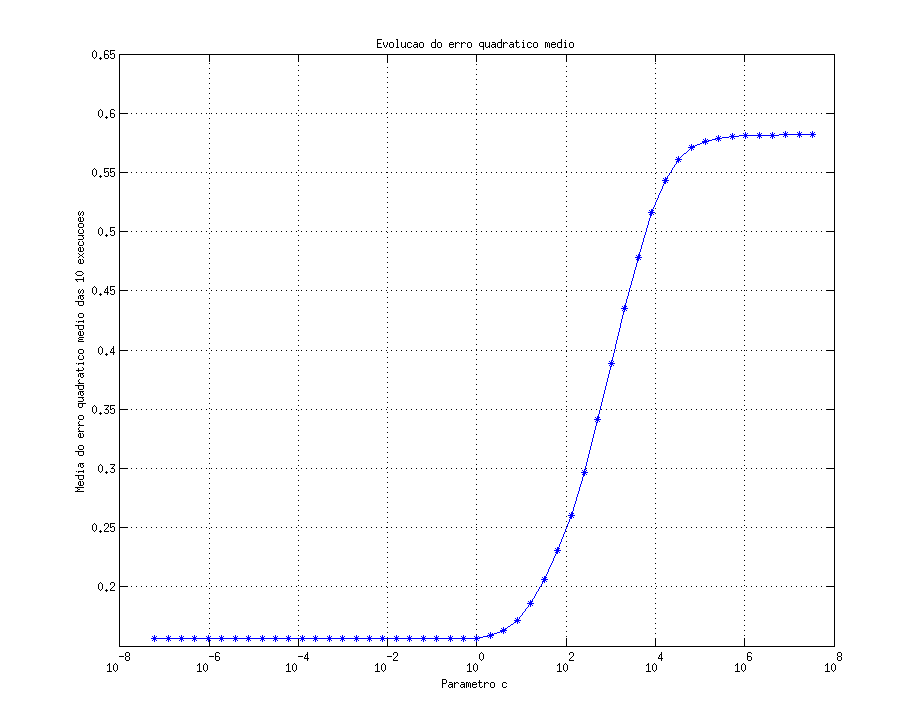
\includegraphics[width=0.65\textwidth]{image/preditor_regularizado_k_folds}
	  \caption{Erro quadrático médio em função do parâmetro c.} 
	  \label{fig:pred.regula}
	\end{figure}
	
	\FloatBarrier 
	
	Ressalta-se a presença de um mínimo local, para \(c_1 = 2^{-1} =
	0.5\), valendo \textbf{0.15602}. Esse erro é inferior a aquele obtido
	ao caso não regularizado, já que o preditor obtido
	neste caso adapta-se melhor a todo conjunto dos dados e não somente a aqueles
	que só foram usados no treinamento.
	
	\vspace{12pt}
	
	Enfim, explicitamos os vetores \(\overrightarrow{b}\) para \(c = 2^{-1}\):
	\FloatBarrier
	\begin {table}[H]
\centering
	\begin{tabular} {| c | c | c | c | c | c | c |}
	\hline 
	\( \overrightarrow{b}_1 \) & -0.1673 & 0.2193 & -0.3182 & -0.0397 & 1.2160 & 
	0.0023 \\\hline 
	\( \overrightarrow{b}_2 \) &-0.1685 & 0.2244 & -0.3230 & -0.0418 & 1.2195 &  0.0014
	\\ \hline 
	\( \overrightarrow{b}_3 \) & -0.1669 & 0.2195 & -0.3199 & -0.0379 & 1.2158 & 
	0.0015 \\ \hline 
	\( \overrightarrow{b}_4 \)  &-0.1674 & 0.2194 & -0.3185 & -0.0390 & 1.2155 & 
	0.0025 \\ \hline
	\( \overrightarrow{b}_5 \) & -0.1680 & 0.2217 & -0.3191 & -0.0400 & 1.2164 & 
	0.0008 \\ \hline 
	\( \overrightarrow{b}_6 \) & -0.1675 & 0.2199 & -0.3191 & -0.0390 & 1.2159 & 
	0.0018 \\ \hline 
	\( \overrightarrow{b}_7 \) & -0.1662 & 0.2329 & -0.3552 & -0.0222 & 1.2199 &
	-0.0014 \\ \hline 
	\( \overrightarrow{b}_8 \) & -0.1676 & 0.2352 & -0.3412 & -0.0347 & 1.2221 & 
	0.0008 \\ \hline 
	\( \overrightarrow{b}_9 \) &-0.1664 & 0.2202 & -0.3225 & -0.0365 & 1.2160 & 
	0.0009 \\ \hline 
	\( \overrightarrow{b}_{10} \) & -0.0832 & -0.0739 & 0.1328 & -0.1357 & 1.0721 &
	-0.0105 \\ \hline
	

	\end{tabular} 
\end {table}

Destaca-se que os valores para as componentes de uma mesma coluna não apresentam
uma grande variação entre si, isto é, os coeficientes do modelo autoregressivo
que produzem o menor erro médio possuem um comportamento bem definido.

\subsection{Síntese de uma rede neural MLP}
\label{sec:mlp}

Os resultados contidos nas seções \ref{sec:iteracoes} e \ref{sec:neuronios}
foram obitdos do programa \texttt{numberNeuronsMLP.m}, contido no trecho de
código \ref{lst:mlp} na seção \textbf{Anexos} no fim deste documento. Em poucas
palavras, este programa automatiza o processo de treinamento de análise dos
resultados de uma rede MLP para diferentes quantidades de neurônios e iterações.
Ele utiliza as funções disponibilizadas pelo professor, que foram adaptadas
somente para receber parâmetros de entrada no lugar de requirir os dados ao
usuário. Neste programa, há dois laços: o mais externo é reponsável por
modificar o número de iterações do algoritmo otimizador, escolhendo valores no
conjunto \(i \in \left\{ 50, 100, 150, 200, 300, 400 \dots 1000 \right\} \) e o
mais interno, o número de neurônios na camada intermediária no conjunto \( n \in
\left\{ 5, 6, 7 \dots 20 \right\} \). Para cada valor de \(i\) e de \(n\)
treina-se 10 MLPs (uma para cada configuração das \textit{folds}) e calcula-se
as médias dos seus desempenhos. Após obtermos as MLPs para todos os valores de \(n\), construimos
um gráfico com as médias dos erros de validação e de teste e, após todos os
valores de \(i\), desenhamos um último gráfico, com os desempenhos médios para
cada valor de \(i\). As próximas seções serão dedicadas às devidas explicações
sobre os resultados.

\subsubsection{Determinação do número de iterações}
\label{sec:iteracoes}

A figura \ref{fig:avg_iter} mostra um gráfico que relaciona o desempenho médio
das MLPs com o número de iterações. Observa-se que os comportamentos dos erros
de teste e de validação são similiares, isto é, quando uma apresenta um valor
elevado, a outra também apresentará. Esta afirmação explica-se pela capacidade
de generalização das MLPs: se uma rede é treinada de forma que o conjunto de
validação seja utilizado, é possível atingir um maior grau de flexibilidade a
todos os dados e, assim, o erro para dados novos não levados em consideração
(como aqueles do conjunto de teste) não se distanciará fortemente do erro de
validação. Sendo assim, utilizaremos o valor que possui o maior custo benefício
entre os dois erros, isto é, \(i = 1000\), que produz um erro médio de validação
igual a \textbf{0.1588} e um erro médio de teste valendo \textbf{0.1813}.

\begin{figure}[H]
			\centering
			  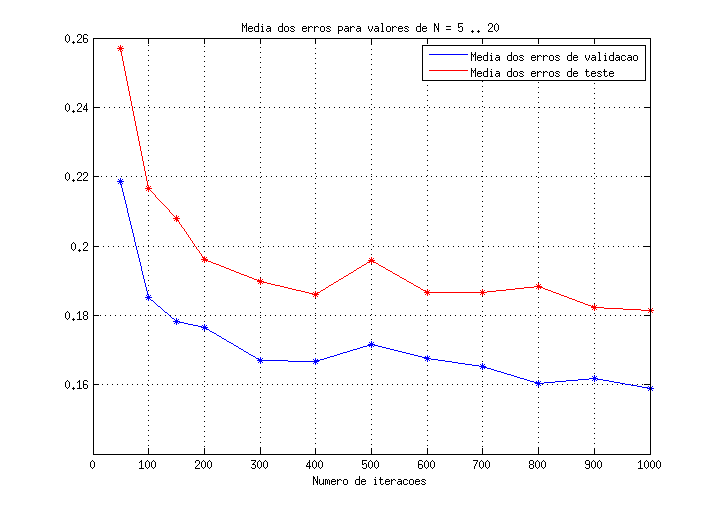
\includegraphics[width=0.650\textwidth]{image/mlp_average_iterations}
			  \caption{Média de todas as MLPs, calculadas para todo valor de \(n\), para
			  cada \(i\).}
			  \label{fig:avg_iter}
	\end{figure}
	
	\FloatBarrier

\subsubsection{Determinação do número de neurônios na camada intermediária}
\label{sec:neuronios}

Uma vez determinado o melhor número de iterações, é possível estabelecer o
número de neurônios que melhor se adequa à aplicação. Para isso, utilizamos o
gráfico da figura \ref{fig:iter1000}.


	\begin{figure}[H]
			\centering
			  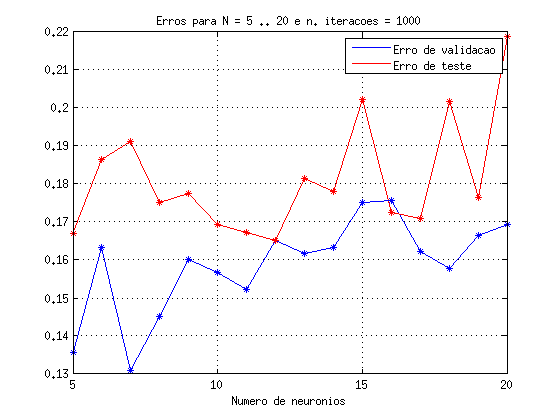
\includegraphics[width=0.650\textwidth]{image/mlp_1000_iterations}
			  \caption{Média de todas as MLPs, calculadas para cada valor de \(n\),
			  para \(i=1000\).}
			  \label{fig:iter1000}
	\end{figure}
	
	\FloatBarrier
	
O melhor custo benefício entre os dois erros é, neste caso \(n = 5\),
apresentando erro médio de validação de \textbf{0.1356} e erro médio de teste de \textbf{0.1671}.
Destaca-se que, para \(n=7\), temos o valor mínimo do erro de validação, mas, ao
mesmo tempo, um erro relacionado ao teste muito elevado. Por esta rezão, este
número de neurônios não foi escolhido.  Observa-se também que as duas curvas não
apresentam comportamentos definidos, isto é, os erros para diferentes valores de
\(n\) são muito distintos entre si.

\vspace{12pt}

Os demais resultados para outros valores de \(i\) e \(n\) podem ser observados
na figura \ref{fig:iens} na seção \textbf{Anexos}. 


\subsection{Síntese da Máquina de Aprendizado Máximo - \textit{ELM}}
\label{sec:elm}

Neste exercício, adotaremos uma \textit{ELM} com apenas uma camada
intermediária com um número de neurônios que determinaremos a seguir. Para tal,
utilizamos o programa \ref{lst:elm}, presente no fim deste documento na seção
\textbf{Anexos}. Neste trecho de código, iteramos o número de neurônios no
conjunto  \( \left\{ 100, 150, 250, 400, 500, 1000  \right\} \) e o parâmetro
regularizador \(c\) e, obtemos um gráfico da média do erro quadrático médio de
validação das 10 execuções (uma para cada \textit{fold}) para valor do número
de neurônios utilizado.

\vspace{12pt}

Após a execução no ambiente MATLAB, encontrou-se que o menor erro quadrático
médio junto ao conjunto de validação foi \textbf{0.3036}, referente a \(N =
400\) neurônios e \(c=2^{-6}=0.015625\). A figura a seguir mostra o resultado da
execução nestas configurações:

	\begin{figure}[H]
			\centering
			  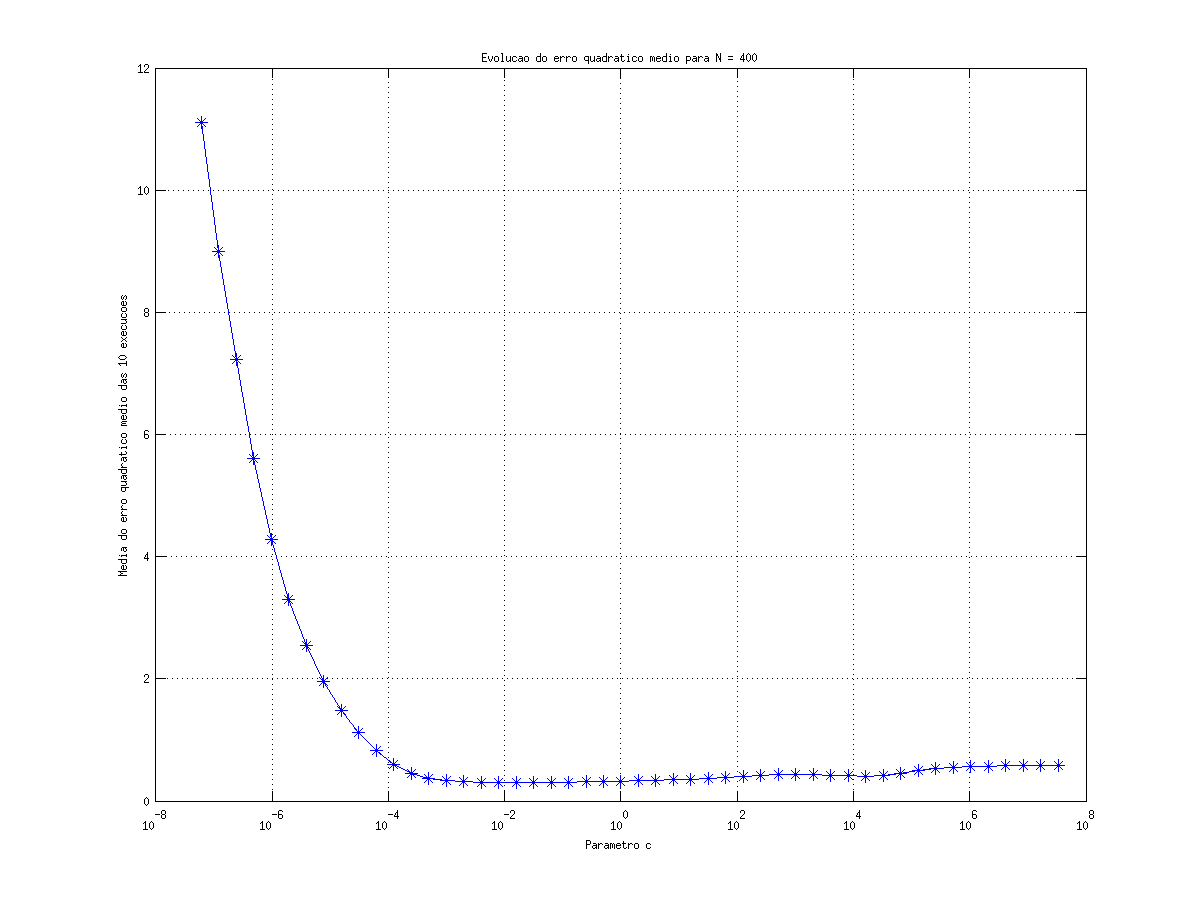
\includegraphics[width=0.650\textwidth]{image/elm_400_neurons}
			  \caption{Erro quadrático médio de validação em função de \(c\),
			  para \(N=400\).}
			  \label{fig:elm400}
	\end{figure}
	
	\FloatBarrier
	
Percebe-se que o erro cresce à medida que \(c\) se aproxima de 0 e depois se
estabiliza para c tendendo a infinito.  Os resultados das demais execuções
encontram-se na figura \ref{fig:elms} na seção \textbf{Anexos}.

\subsection{Análise dos resultados dos preditores lineares, MLPs e ELMs}
\label{sec:comparacao}

A pior performance entre os quatro preditores implementados nesta lista foi a
do \textit{ELM}, que obteve um erro quadrático médio de \textbf{0.3036}. Tal
resultado é um tanto quanto surpreendente, já que esse desempenho é inferior a
aquele dos preditores lineares, fato este que não era esperado.  Possíveis
explicações para este fato são a quantidade insuficiente de camadas utilizadas,
a inicialização dos pesos sinápticos da camada intermediária, que, foi neste
caso, determinada aleatoriamente segundo uma lei normal de média 0 e variância
1, ou algum erro eventual no programa \ref{lst:elm}.

\vspace{12pt}

O terceiro lugar, \textit{preditor linear não regularizado}, para qual só foi
utilizado o conjunto de treinamento para o cálculo do erro quadrático médio,
obteve um erro de \textbf{0.2500}. Uma vez o conjunto de validação não foi
utilizado, a capacidade de generalização do preditor é comprometido e, assim, o
preditor apresenta um erro relativamente alto.

\vspace{12pt}

Em segundo lugar, destaca-se \textit{preditor linear regularizado}, cujo erro
quadrático médio vale \textbf{0.15602}. A introdução de um parâmetro \(c\) adicional e a
sua determinação ótima juntamente ao conjunto de validação provaram que o
desempenho obtido pode ser melhorado de maneira significativa, visto que o
modelo linear mantem-se o mesmo. Isso significa que nesta oportunidade,
observa-se uma maior flexibilidade do preditor a todos os dados.

\vspace{12pt}  

Enfim, para o caso das MLPs, obtem-se um erro médio quadrático de validação de
\textbf{0.1356}, para \(i=1000\) e \(n=5\). É necessário dizer que este resultado foi
conseguido com base em uma quantidade de processamento muito superior aos dois
casos precedentes, uma vez que, no total, foram treinadas
\(10*\mathbf{card}(n)*\mathbf{card}(i) = 10*15*12 = 1800\) MLPs (uma para cada
configuração das \textit{folds}, cada valor de \(n\) e \(i\)). Foram utilizados
conjuntos de validação e teste para otimizar ainda mais a adequação da rede aos
dados. A rede neural é, portanto, a melhor opção para predizer a série temporal
da dengue em São Paulo.

\section{Conclusao}

\section* {Referências bibliográficas}
\begin {itemize}
  \item \url{https://en.wikipedia.org/wiki/Sunspot}. Acessado às 19:22 29/09/2015.
  \item Guyon, I.; Elisseeff, A. "An introduction to variable and feature selection", Journal of Machine Learning Resear ch, vol. 3, pp. 1157 - 1182 2003.
  \item \url{http://archive.ics.uci.edu/ml/datasets/Wine+Quality}.\\
  	 Acessado às 21:27 30/09/2015.
\end{itemize}

\newpage

\section{Anexos}

\subsection {Programas}

\lstinputlisting [language=Matlab, caption={ \texttt{gera\_dados.m} - cria a
		sequência temporal.}, label={lst:geracao}] {predicao/gera_dados.m}
		
\lstinputlisting [language=Matlab, caption={
\texttt{resolve\_sistema\_k\_folds.m} - calcula preditores lineares.},
label={lst:preditor}] {predicao/resolve_sistema_k_folds.m}

\lstinputlisting [language=Matlab, caption={ 
\texttt{numberNeuronsMLP.m} - Automatiza treinamento e análise de redes MLP.},
label={lst:mlp}] {predicao/numberNeuronsMLP.m}

\lstinputlisting [language=Matlab, caption={ 
\texttt{elm.m} - Automatiza treinamento e análise de redes \textit{ELMs}.},
label={lst:elm}] {predicao/elm.m}
		
\FloatBarrier

\newpage

\subsection {Figuras}

A figura \ref{fig:forw} possui todos os resultados das execuções do
\textit{forward selection} para a série dos \textit{sunspots}. Observa-se que o
comportamento das curvas em todas elas é muito parecido, apresentando um mínimo para um número de variáveis
próximo de 15. \textit{(Rever análise completa na seção 2 item
\ref{item:forwsunspot}).}

\FloatBarrier
\begin{figure}[H] 
				
			\centering
			
				\begin{subfigure}{.5\textwidth}
				  \centering
				  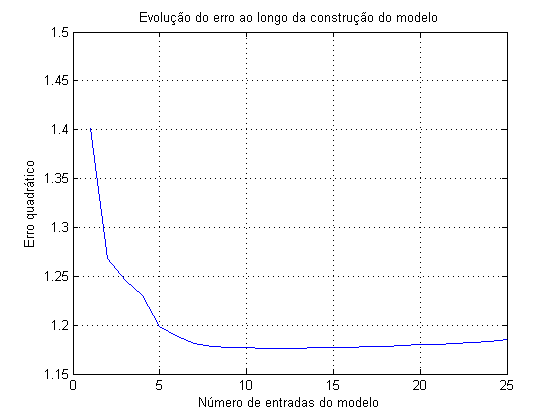
\includegraphics[width=1\linewidth]{image/forward1}
				  \caption{Resultado da execução 1.}
				  \label{forward1}
				\end{subfigure}%
				\begin{subfigure}{.5\textwidth}
				  \centering
				  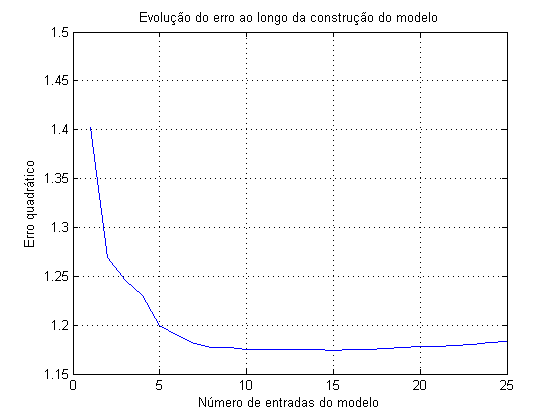
\includegraphics[width=1\linewidth]{image/forward2}
				  \caption{Resultado da execução 2.}
				  \label{forward2}
			\end{subfigure}
			
			\begin{subfigure}{.5\textwidth}
				  \centering
				  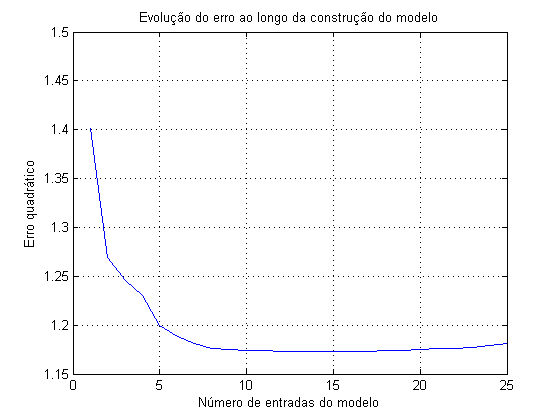
\includegraphics[width=1\linewidth]{image/forward3}
				  \caption{Resultado da execução 3.}
				  \label{forward3}
				\end{subfigure}%
				\begin{subfigure}{.5\textwidth}
				  \centering
				  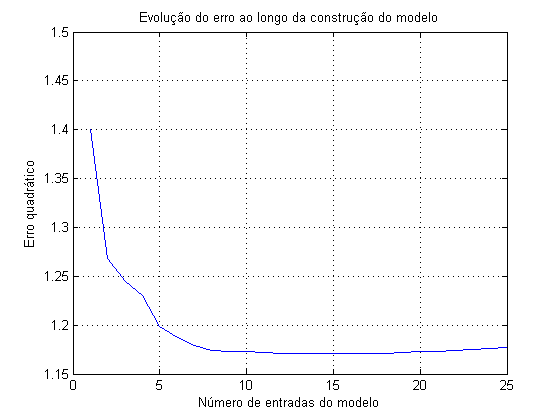
\includegraphics[width=1\linewidth]{image/forward4}
				  \caption{Resultado da execução 4.}
				  \label{forward4}
				\end{subfigure}			
			
			\begin{subfigure}{.5\textwidth}
				  \centering
				  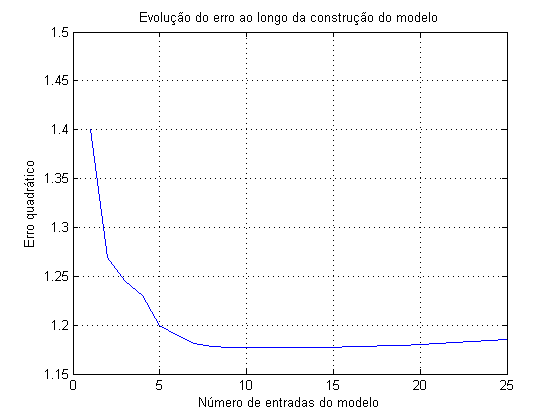
\includegraphics[width=1\linewidth]{image/forward5}
				  \caption{Resultado da execução 5.}
				  \label{forward5}
				\end{subfigure}	
			
			\caption{Resultados das execuções da \textit{forward selection} para os
			dados de \texttt{sunspot.mat}.}
			\label{fig:forw}
			\end{figure}
			
		\FloatBarrier


A figura \ref{fig:back} possui todos os resultados das
execuções do \textit{backward elimination} para a série dos \textit{sunspots}.
Assim como o caso anterior, observa-se que o comportamento das curvas em todas elas é muito
parecido, apresentando um mínimo para um número de variáveis próximo de 15.
\textit{(Rever análise completa na seção 2 item \ref{item:forwsunspot}).}
		
		\begin{figure}[H] 
				
			\centering
			
				\begin{subfigure}{.5\textwidth}
				  \centering
				  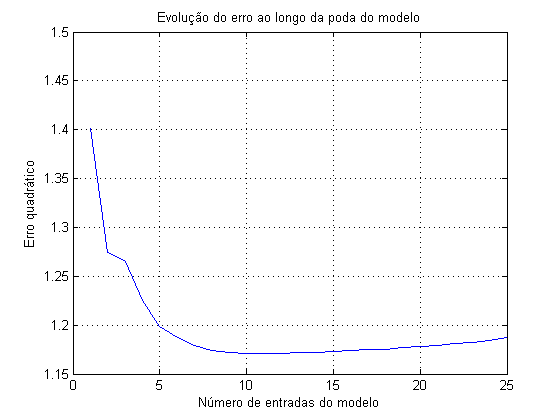
\includegraphics[width=1\linewidth]{image/backward1}
				  \caption{Resultado da execução 1.}
				  \label{backward1}
				\end{subfigure}%
				\begin{subfigure}{.5\textwidth}
				  \centering
				  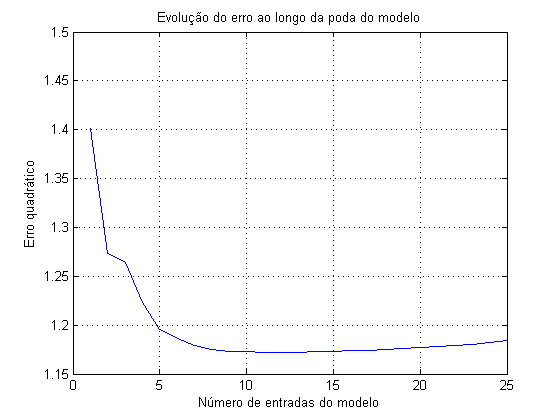
\includegraphics[width=1\linewidth]{image/backward2}
				  \caption{Resultado da execução 2.}
				  \label{backward2}
			\end{subfigure}
			
			\begin{subfigure}{.5\textwidth}
				  \centering
				  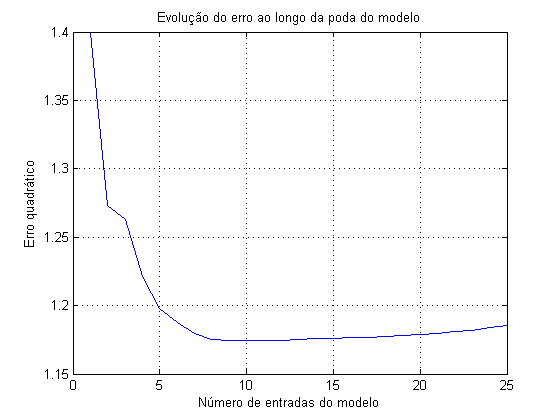
\includegraphics[width=1\linewidth]{image/backward3}
				  \caption{Resultado da execução 3.}
				  \label{backward3}
				\end{subfigure}%
				\begin{subfigure}{.5\textwidth}
				  \centering
				  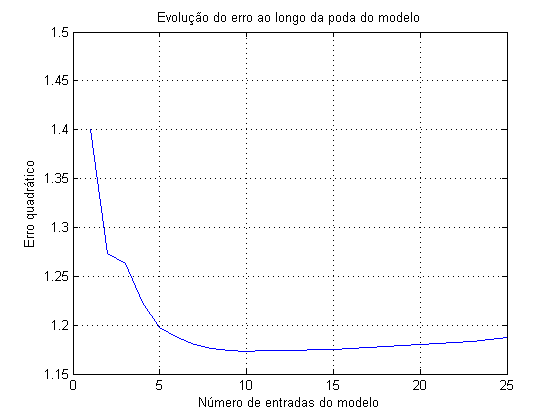
\includegraphics[width=1\linewidth]{image/backward4}
				  \caption{Resultado da execução 4.}
				  \label{backward4}
				\end{subfigure}			
			
			\begin{subfigure}{.5\textwidth}
				  \centering
				  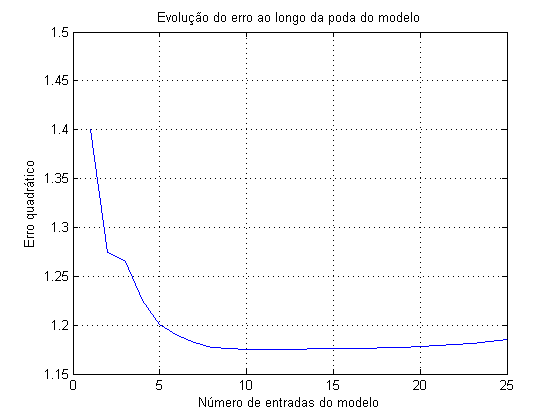
\includegraphics[width=1\linewidth]{image/backward5}
				  \caption{Resultado da execução 5.}
				  \label{backward5}
				\end{subfigure}	
			
			\caption{Resultados das execuções da \textit{backward elimination} para os
			dados de \texttt{sunspot.mat}.}
			\label{fig:back}
			\end{figure}


\FloatBarrier

\newpage

A figura \ref{fig:forw2} possui todos os resultados das
execuções do \textit{forward selection} para os dados contidos em
\texttt{wineq.mat}. Observa-se que o comportamento das curvas em todas elas é
muito parecido, apresentando um mínimo para um número de variáveis próximo de 8.
\textit{(Rever análise completa na seção 2 item \ref{item:forwwineq}).}

\begin{figure}[H] 
				
			\centering
			
				\begin{subfigure}{.5\textwidth}
				  \centering
				  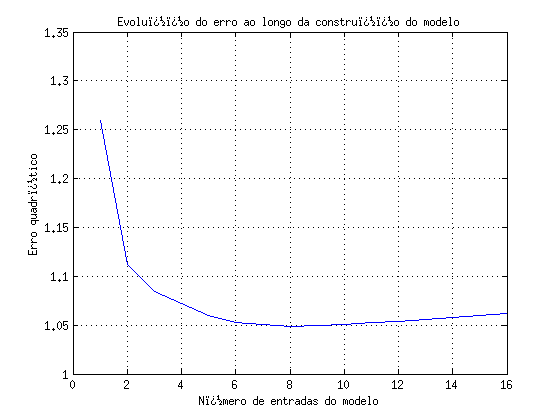
\includegraphics[width=1\linewidth]{image/forward1_2}
				  \caption{Resultado da execução 1.}
				  \label{forward1_2}
				\end{subfigure}%
				\begin{subfigure}{.5\textwidth}
				  \centering
				  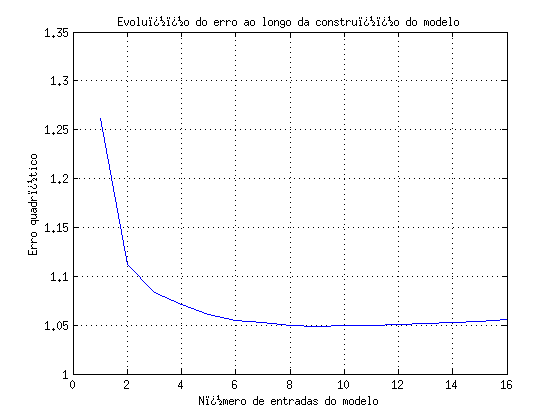
\includegraphics[width=1\linewidth]{image/forward2_2}
				  \caption{Resultado da execução 2.}
				  \label{forward2_2}
			\end{subfigure}
			
			\begin{subfigure}{.5\textwidth}
				  \centering
				  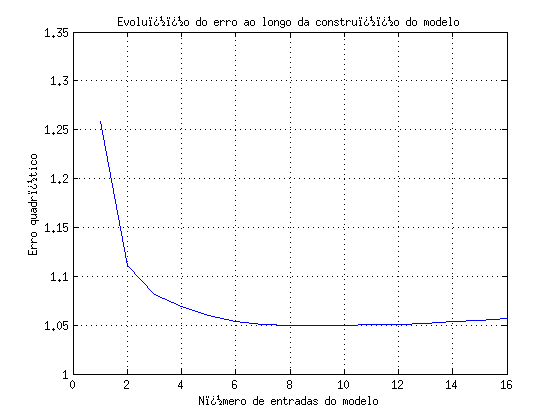
\includegraphics[width=1\linewidth]{image/forward3_2}
				  \caption{Resultado da execução 3.}
				  \label{forward3_2}
				\end{subfigure}%
				\begin{subfigure}{.5\textwidth}
				  \centering
				  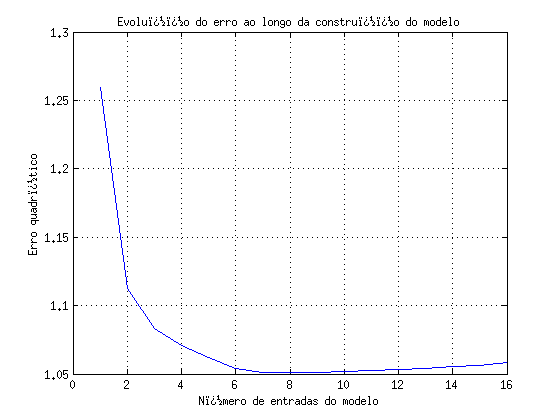
\includegraphics[width=1\linewidth]{image/forward4_2}
				  \caption{Resultado da execução 4.}
				  \label{forward4_2}
				\end{subfigure}			
			
			\begin{subfigure}{.5\textwidth}
				  \centering
				  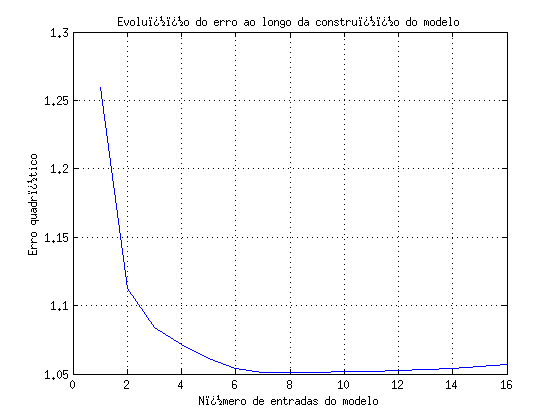
\includegraphics[width=1\linewidth]{image/forward5_2}
				  \caption{Resultado da execução 5.}
				  \label{forward5_2}
				\end{subfigure}	
			
			\caption{Resultados das execuções da \textit{forward selection} para os
			dados de \texttt{wineq.mat}.}
			\label{fig:forw2}
			\end{figure}
			
		\FloatBarrier

\newpage

A figura \ref{fig:back2} possui todos os resultados das
execuções do \textit{backward elimination} para os dados contidos em
\texttt{wineq.mat}. Observa-se que o comportamento das curvas em todas elas é
muito parecido, apresentando um mínimo para um número de variáveis próximo de
10. \textit{(Rever análise completa na seção 2 item \ref{item:forwwineq}).}	
		
		\begin{figure}[H] 
				
			\centering
			
				\begin{subfigure}{.5\textwidth}
				  \centering
				  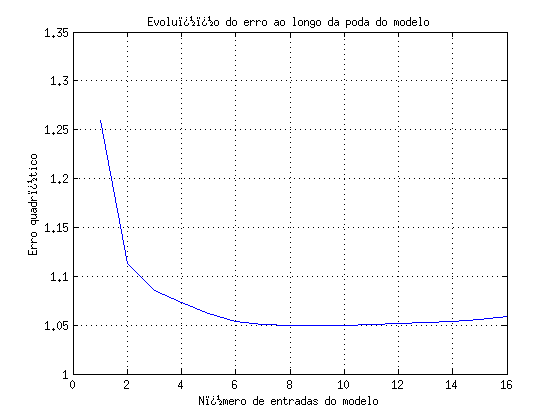
\includegraphics[width=1\linewidth]{image/backward1_2}
				  \caption{Resultado da execução 1.}
				  \label{backward1_2}
				\end{subfigure}%
				\begin{subfigure}{.5\textwidth}
				  \centering
				  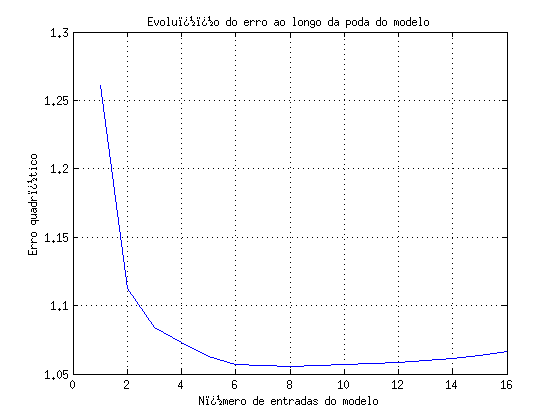
\includegraphics[width=1\linewidth]{image/backward2_2}
				  \caption{Resultado da execução 2.}
				  \label{backward2_2}
			\end{subfigure}
			
			\begin{subfigure}{.5\textwidth}
				  \centering
				  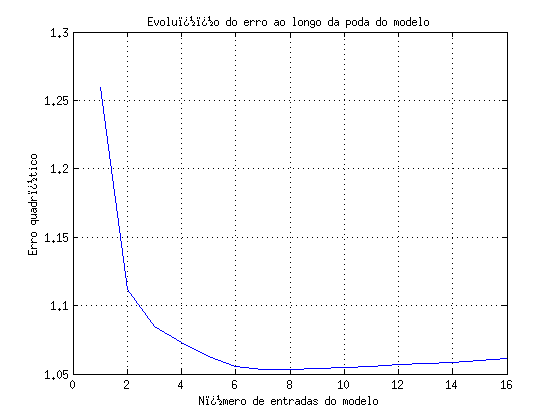
\includegraphics[width=1\linewidth]{image/backward3_2}
				  \caption{Resultado da execução 3.}
				  \label{backward3_2}
				\end{subfigure}%
				\begin{subfigure}{.5\textwidth}
				  \centering
				  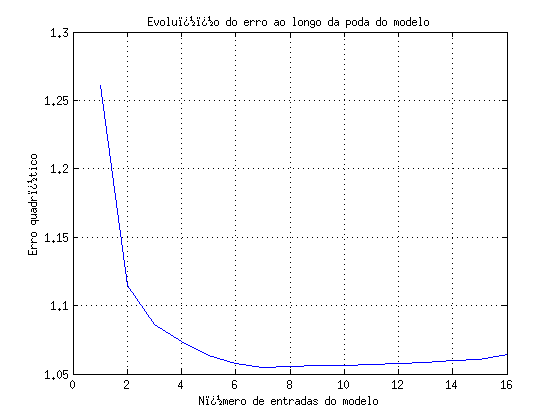
\includegraphics[width=1\linewidth]{image/backward4_2}
				  \caption{Resultado da execução 4.}
				  \label{backward4_2}
				\end{subfigure}			
			
			\begin{subfigure}{.5\textwidth}
				  \centering
				  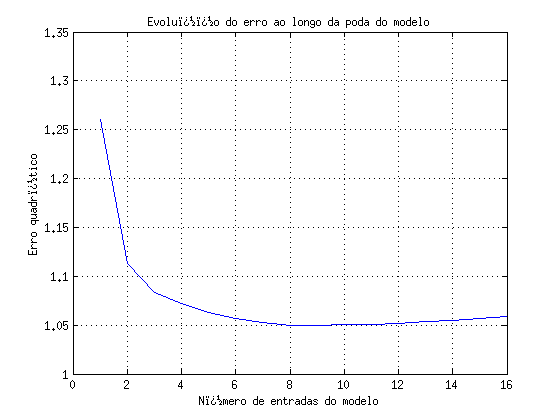
\includegraphics[width=1\linewidth]{image/backward5_2}
				  \caption{Resultado da execução 5.}
				  \label{backward5_2}
				\end{subfigure}	
			
			\caption{Resultados das execuções da \textit{backward elimination} para os
			dados de \texttt{wineq.mat}.}
			\label{fig:back2}
			\end{figure}
			
		\FloatBarrier
				
		
		
\newpage

Resultados obtidos para diversos valores do número de iterações do algoritmo
otimizador. Destaca-se que os resultados não apresentam nenhum comportamento bem
definido, mas tendem a diminuir com o aumento de \(i\). \textit{(Rever análise
completa na seção
\ref{sec:iteracoes}.)}
		
		\begin{figure}[H] 
				
			\centering
			
				\begin{subfigure}{.33\textwidth}
				  \centering
				  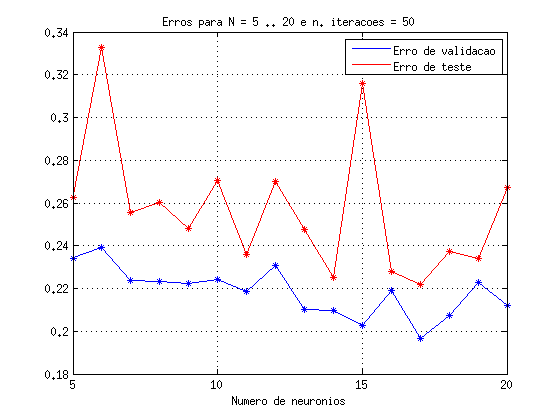
\includegraphics[width=1\linewidth]{image/mlp_50_iterations}
				  \caption{\(i=50\).}
				\end{subfigure}%
				\begin{subfigure}{.33\textwidth}
				  \centering
				  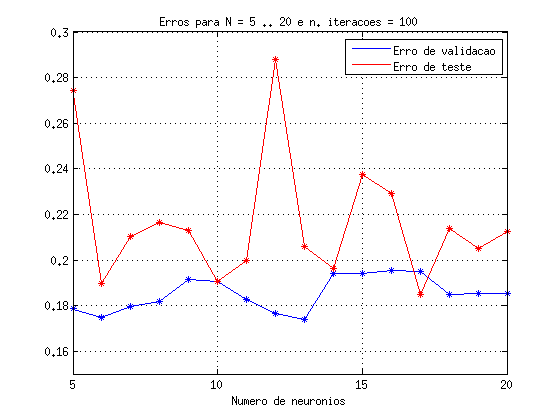
\includegraphics[width=1\linewidth]{image/mlp_100_iterations}
				  \caption{\(i=100\).}
			\end{subfigure}
			\begin{subfigure}{.33\textwidth}
				  \centering
				  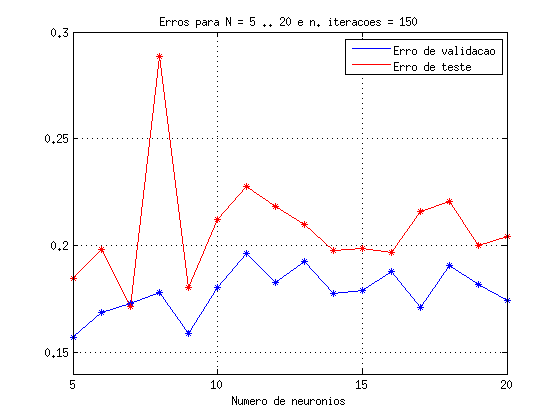
\includegraphics[width=1\linewidth]{image/mlp_150_iterations}
				  \caption{\(i=150\).}
				\end{subfigure}%
				
				\begin{subfigure}{.33\textwidth}
				  \centering
				  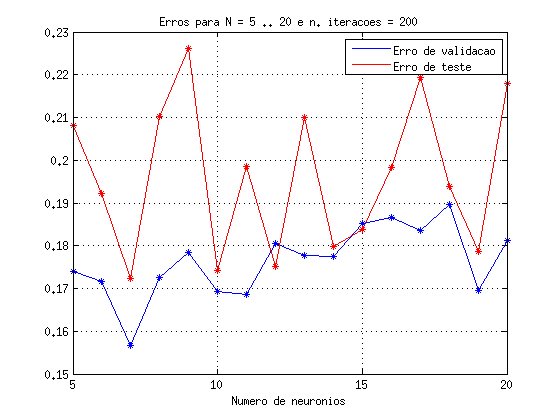
\includegraphics[width=1\linewidth]{image/mlp_200_iterations}
				  \caption{\(i=200\).}
				\end{subfigure}%
				\begin{subfigure}{.33\textwidth}
				  \centering
				  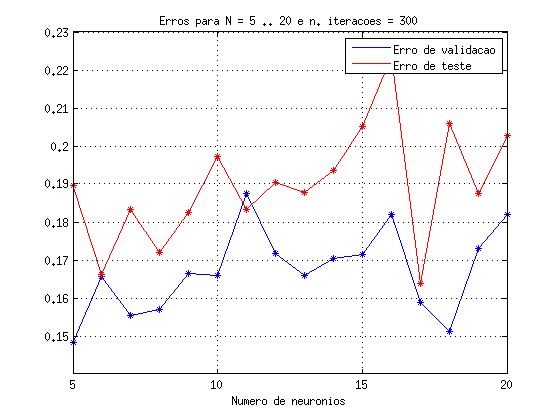
\includegraphics[width=1\linewidth]{image/mlp_300_iterations}
				  \caption{\(i=300\).}
			\end{subfigure}
			\begin{subfigure}{.33\textwidth}
				  \centering
				  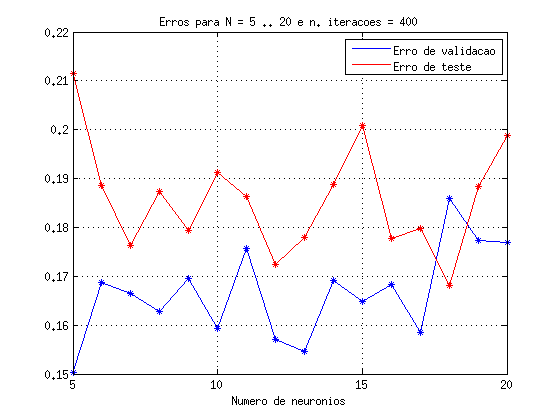
\includegraphics[width=1\linewidth]{image/mlp_400_iterations}
				  \caption{\(i=400\).}
				\end{subfigure}%	
				
			\begin{subfigure}{.33\textwidth}
				  \centering
				  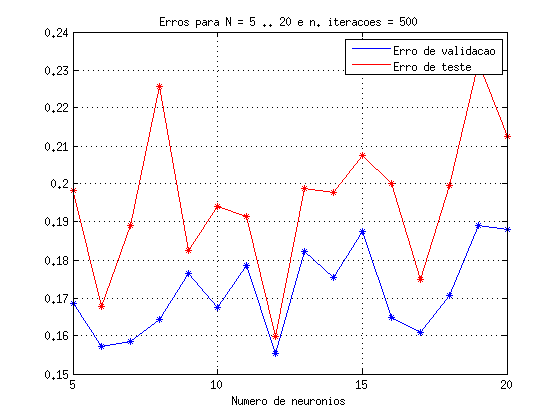
\includegraphics[width=1\linewidth]{image/mlp_500_iterations}
				  \caption{\(i=500\).}
				\end{subfigure}%
				\begin{subfigure}{.33\textwidth}
				  \centering
				  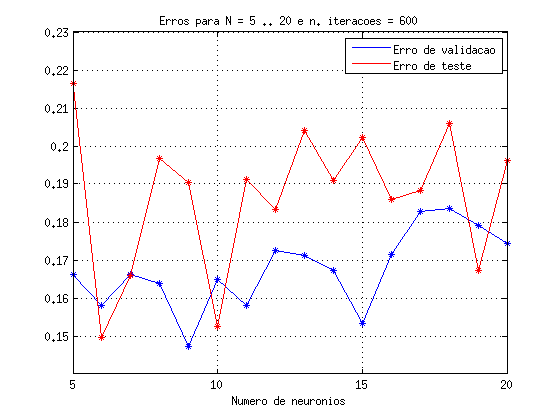
\includegraphics[width=1\linewidth]{image/mlp_600_iterations}
				  \caption{\(i=600\).}
			\end{subfigure}
			\begin{subfigure}{.33\textwidth}
				  \centering
				  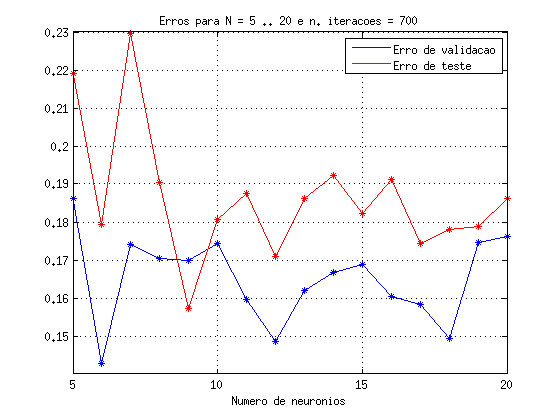
\includegraphics[width=1\linewidth]{image/mlp_700_iterations}
				  \caption{\(i=700\).}
				\end{subfigure}%
			
			\begin{subfigure}{.5\textwidth}
				  \centering
				  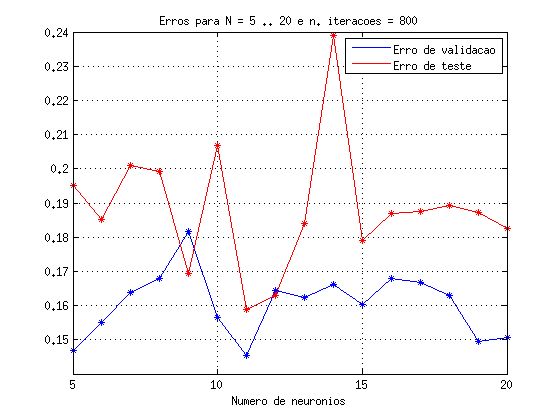
\includegraphics[width=1\linewidth]{image/mlp_800_iterations}
				  \caption{\(i=800\).}
				\end{subfigure}%
				\begin{subfigure}{.5\textwidth}
				  \centering
				  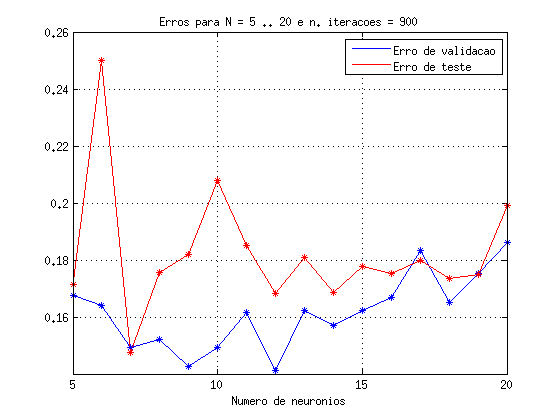
\includegraphics[width=1\linewidth]{image/mlp_900_iterations}
				  \caption{\(i=900\).}
			\end{subfigure}
			
			\caption{Médias dos erros de validação e de
			teste para vários valores possíveis \(i\) de iteração.}
			\label{fig:iens}
			\end{figure}
			
		\FloatBarrier
		
	
		\newpage
		
		Observa-se que, para valores de \(c\) que tendem a
		0, as ELMs produzem um grande erro quadrático médio junto aos dados de
		validação. Nota-se também que o erro tende a se estabilizar para \(c\) muito
		grande.
				
		
		\begin{figure}[H] 
				
			\centering
			
				\begin{subfigure}{.5\textwidth}
				  \centering
				  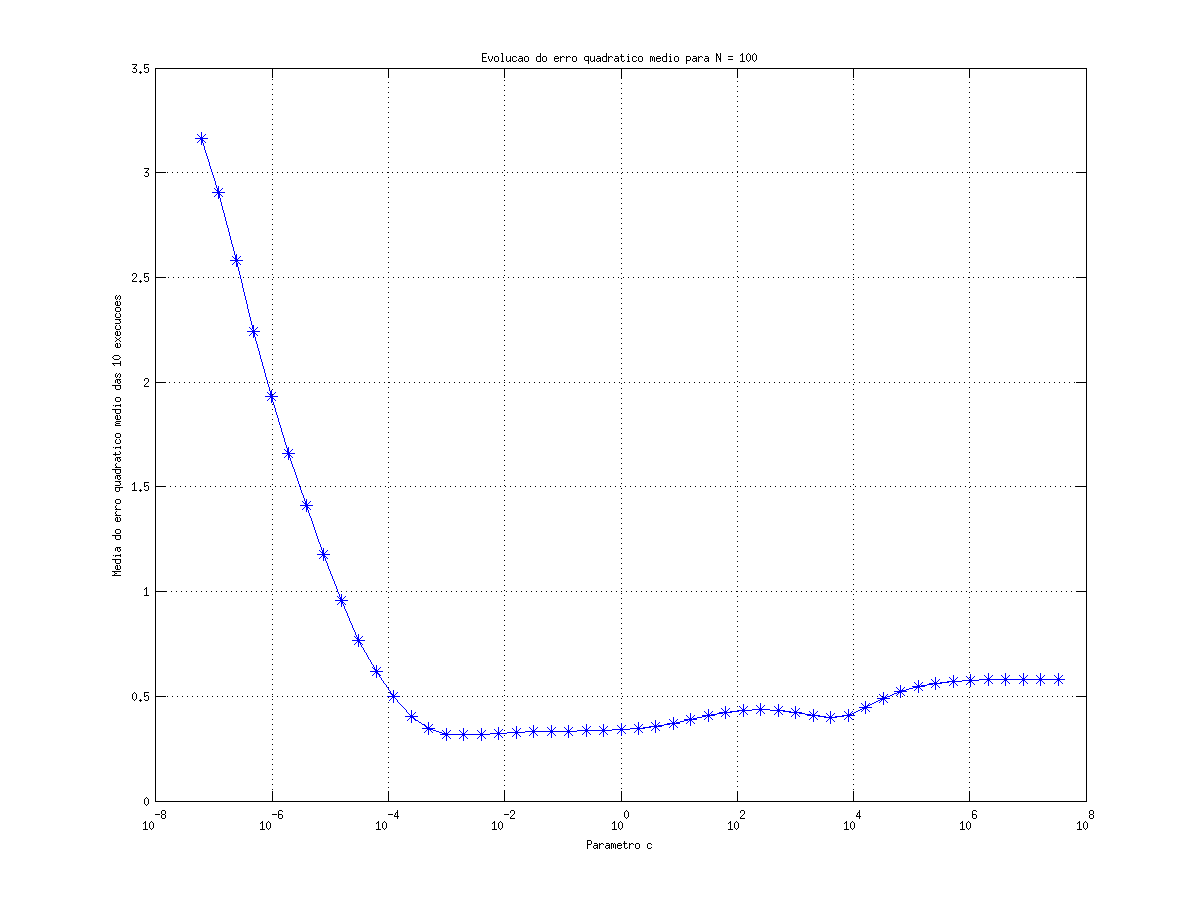
\includegraphics[width=1\linewidth]{image/elm_100_neurons}
				  \caption{\(N=100\)}
				  \label{fig:elm100}
				\end{subfigure}%
				\begin{subfigure}{.5\textwidth}
				  \centering
				  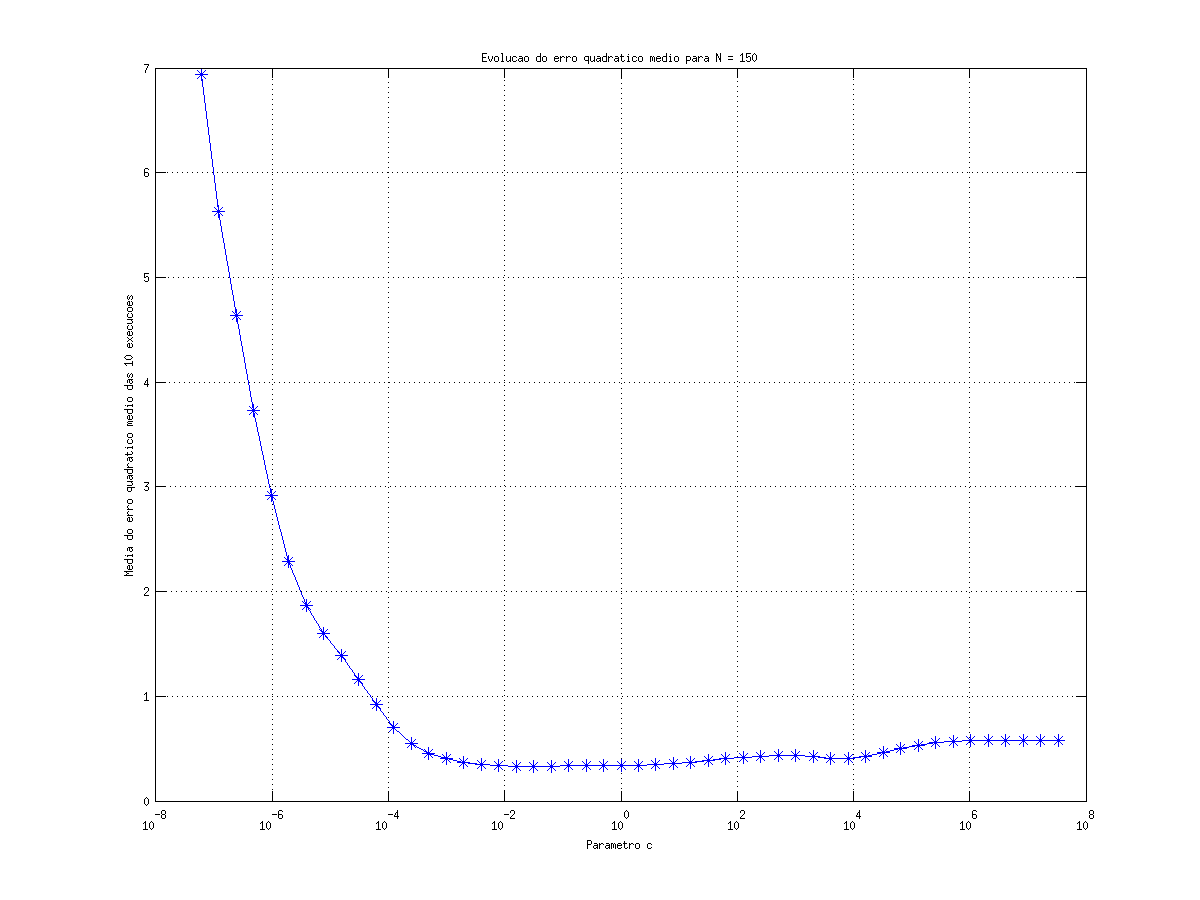
\includegraphics[width=1\linewidth]{image/elm_150_neurons}
				  \caption{\(N=150\)}
				  \label{fig:elm150}
			\end{subfigure}
			
			\begin{subfigure}{.5\textwidth}
				  \centering
				  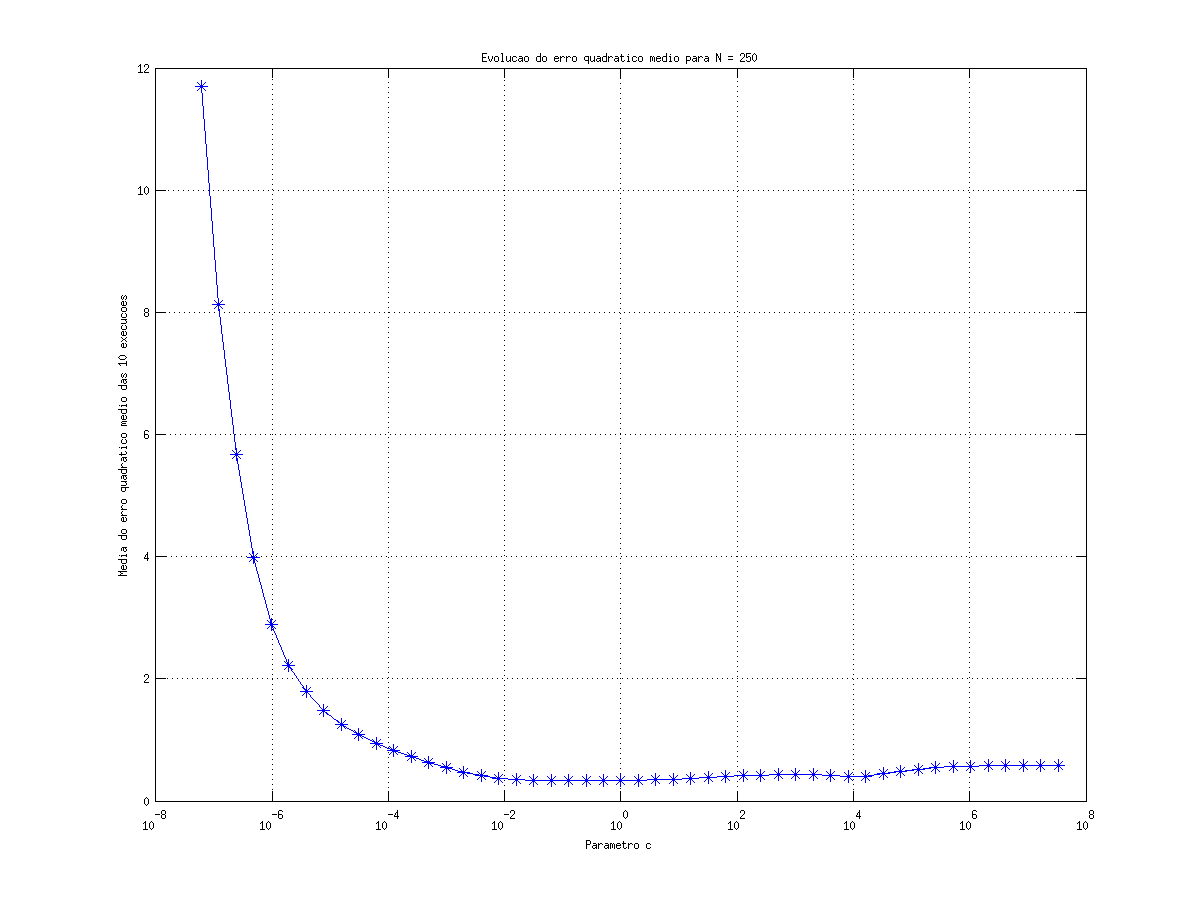
\includegraphics[width=1\linewidth]{image/elm_250_neurons}
				  \caption{\(N=250\)}
				  \label{fig:elm250}
				\end{subfigure}%
				\begin{subfigure}{.5\textwidth}
				  \centering
				  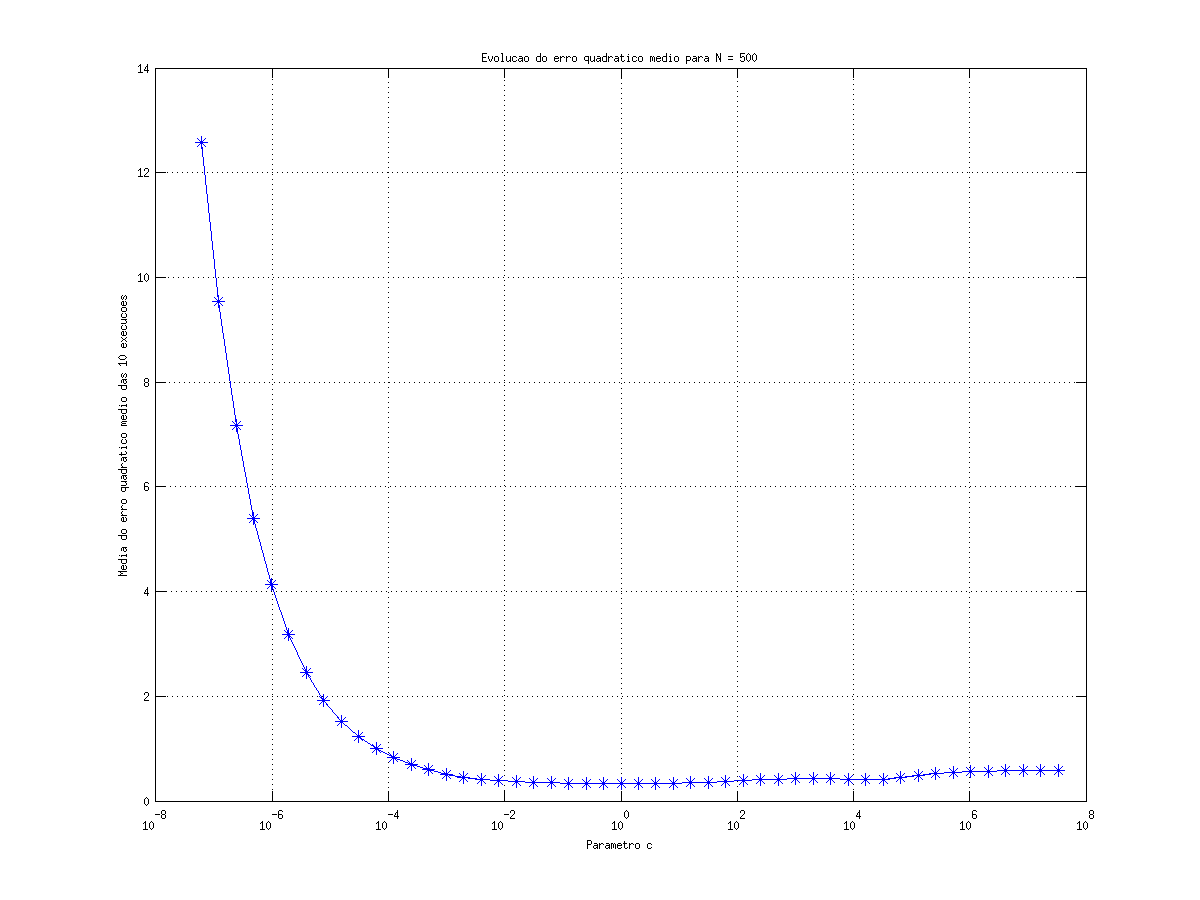
\includegraphics[width=1\linewidth]{image/elm_500_neurons}
				  \caption{\(N=500\)}
				  \label{fig:elm500}
				\end{subfigure}			
			
			\begin{subfigure}{.5\textwidth}
				  \centering
				  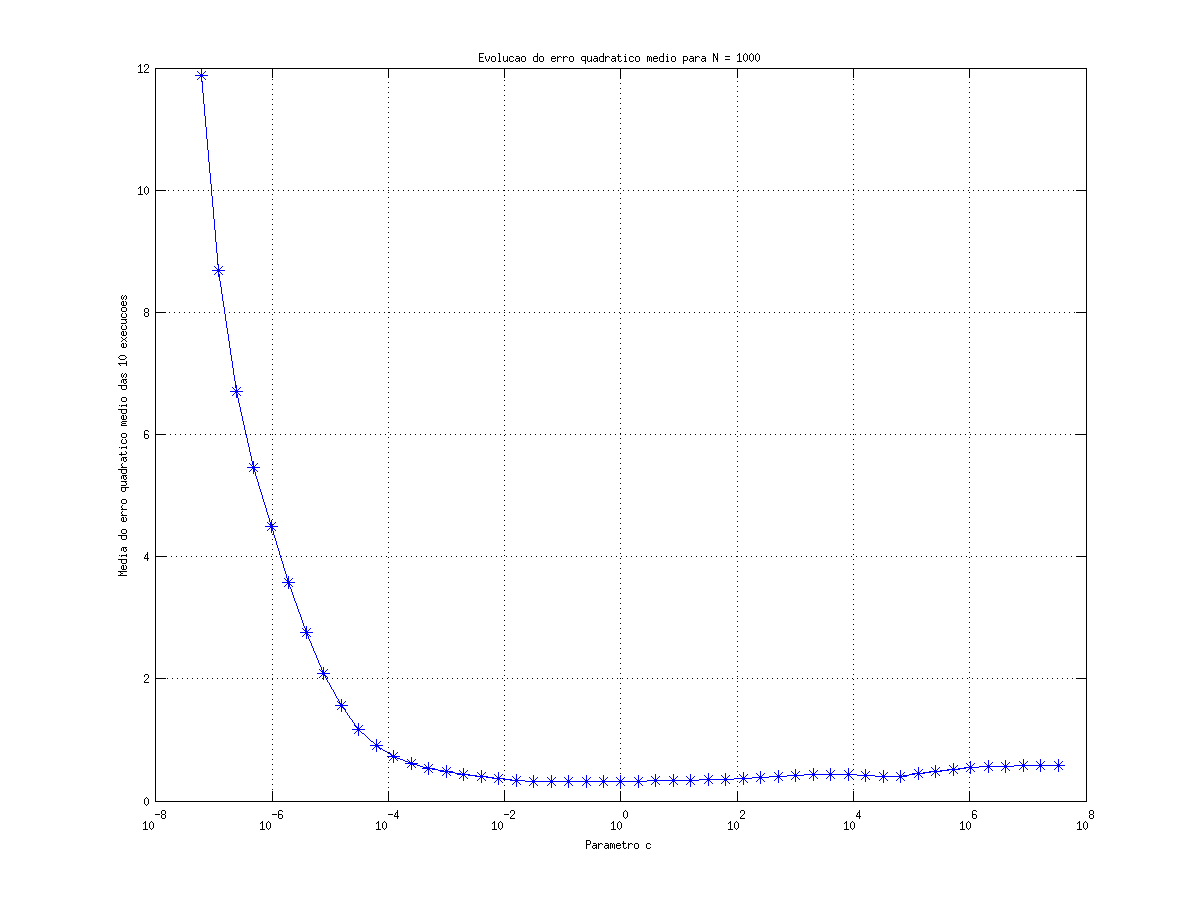
\includegraphics[width=1\linewidth]{image/elm_1000_neurons}
				  \caption{\(N=1000\)}
				  \label{fig:elm1000}  
				\end{subfigure}	
			
			\caption{Resultados das execuções de treinamento e validação de ELMs para diversos números de neurônios.}
			\label{fig:elms}
			\end{figure}
			
		\FloatBarrier
    
\end{document}
